\documentclass[accentcolor=tud1c,longdoc,nopartpage,table,oneside,bibtotoc, liststotoc,openright,colorbacktitle,inverttitle,numbersubsubsec,noresetcounter,11pt,noheadingspace,numbers=noenddot,article,parskip=half]{tudreport}

% Babel-Paket f. neue deutsche Rechtschreibung
\usepackage[ngerman]{babel}
\usepackage{graphicx}
% Eingabekodierung auf latin1 setzen
\usepackage[utf8]{inputenc}


% Font-Encoding auf T1 setzen
\usepackage[T1]{fontenc}
% footmisc behebt u.a. Probleme mit Fu�noten in Abschnittstiteln
\usepackage[stable]{footmisc}

% Einbinden von Grafiken erm�glichen
\usepackage{graphicx}

\usepackage{newunicodechar}
\newunicodechar{ß}{\ss}
% Paket xtab erm�glicht Umbrechen von langen Tabellen
\usepackage{xtab}

% picins erlaubt das Umflie�en von Abbildungen durch Text
% Untenstehendes renewcommand behebt den picins-bug, dass Abbildungen
% nicht im Abbildungsverzeichnis auftauchen
\usepackage{picins}
\makeatletter
\renewcommand\piccaption{\@dblarg{\@piccaption}}
\makeatother

\usepackage{verbatim}

% Einr�ckung bei Zeilenumbruch vermeiden
\setlength{\parindent}{0pt}
\setlength{\parskip}{9pt}
% Tiefe des Inhaltsverzeichnis (paragraphen werden mit aufgenommen)
\setcounter{secnumdepth}{4}
\setcounter{tocdepth}{4}
%Überschriften 
%\addtokomafont{subsection}{\normalsize\bf}
\addtokomafont{subsection}{\normalsize\normalfont\bfseries}
\addtokomafont{subsubsection}{\normalsize\normalfont\bfseries}
\addtokomafont{paragraph}{\small\normalfont\bfseries}


%Silbentrennung von zusammengesetzten w�rtern
\usepackage[ngerman=ngerman-x-latest]{hyphsubst}
% Paket setspace erlaubt Umschalten auf 1.5fachen Zeilenabstand
\usepackage{setspace}


%%%%%%%%%%%%%%%%%%%%%%%%%%%%%%%%%%%%%%%%%%%%%%%%%%%%%%%%
%% Anpassungen von Literaturverzeichnis und Zitierweise%
\usepackage[hyphens]{url}
\usepackage[commabeforerest,authorformat=year,see,dotafter=bibentry,pages=format]{jurabib} % , ibidem=strict 
%\AddTo\bibsgerman{%
%\renewcommand*{\ibidemname}{ebd.}
%\renewcommand*{\ibidemmidname}{ebd.}
%}
%Trennzeichen zwischen Autoren im Zitat

%\AddTo\bibsgerman{%
%\def\jbpagename{S.}%
%\def\jbpagesname{S}%
%}

\renewcommand*{\jbbtasep}{ \& }
\renewcommand*{\jbbfsasep}{; }
\renewcommand*{\jbbstasep}{; }

%Trennzeichen zwischen Autoren im Literaturverzeichnis
\renewcommand*{\bibbtasep}{ \& }
\renewcommand*{\bibbfsasep}{; }
\renewcommand*{\bibbstasep}{ \& }

%Trennzeichen zwischen Herausgebern im Literaturverzeichnis
\renewcommand*{\bibbtesep}{; }
\renewcommand*{\bibbfsesep}{; }
\renewcommand*{\bibbstesep}{; }

%Unterdr�ckt, dass bei mehr als drei Autoren im Literaturverzeichnis
%mit "et al." abgek�rzt wird --> myjureco.bst-Datei wird zus�zlich ben�tigt!
\makeatletter
\def\jb@use@fullcite{%
\jbauthorfont{\jb@@author}\normalfont{\jbhowsepbeforetitle}\jb@@fulltitle}%
\makeatother

%In: erscheint vor dem Titel von Zeitschriften, Konferenzbeitr�gen, Sammelwerken
%und Herausgeberb�nden
%\AddTo\bibsall{\def\incollinname{\textbf{In:}}}
\renewcommand{\bibbtsep}{In: }
\renewcommand*{\bibjtsep}{In: }

%Vor- und Nachname des Herausgebers werden nicht fett gedruckt
\renewcommand*{\biblnfont}{} 
\renewcommand*{\bibfnfont}{}

%�ndert bei urldate das Pr�fix von "Zugriff am" zu "Abruf am"
\AddTo\bibsgerman{\renewcommand*{\urldatecomment}{Letzter Abruf: }}

%Setzt ein Komma zwischen der URL und "Abruf am"
\renewcommand*{\bibbudcsep}{, }

%Entfernt die Zeichen vor und nach der URL-Angabe im Literaturverzeichnis
\renewcommand*{\biburlprefix}{}
\renewcommand*{\biburlsuffix}{}

%Entfernt das Komma zwischen Jahrgang und Ausgabe
%und setzt die Ausgabe in Klammern
\renewcommand*\artnumberformat[1]{\unskip\space (#1)}

%Entfernt das Komma zwischen Adresse und Verlag
%und setzt daf�r ein Leerzeichen. Dies ist n�tig,
%da die Reihenfolge von Adresse und Verlag in myjureco vertauscht wird
%und kein Zeichen nach der Adresse erscheinen soll.
\renewcommand*\bpubaddr{}
\renewcommand*{\bibtfont}{\textit}
% Check if this gives errors
\renewcommand*{\bibapifont}{\textit}
\renewcommand*{\bibatsep}{,}
\renewcommand*{\ajtsep}{,}

%%%%%%%%%%%%%%%%%%%%%%%%%%%%%%%%%%%%%%%%%%%%%%%%%%%%%%%%


\usepackage{hyperref}
%Erm�glicht Hyperlinks zwischen Textstellen und zu externen Dokumenten
%% breaklinks=true/false: Gibt an, ob Links umgebrochen werden d�rfen.
%% linktocpage=true/false: im Inhaltsverzeichnis sind nur die Seitenzahlen
%% links, nicht der Text
%% colorlinks=true/false: Links werden eingef�rbt (Farben werden mit
%% linkcolor, anchorcolor \dots festgelegt)
%% linkcolor=Farbe: Farbe des verlinkten Textes, Dokument-interne Links
%% citecolor=Farbe: Farbe des verlinkten Textes, Links zum
%% Literaturverzeichnis
%% filecolor=Farbe: Farbe des verlinkten Textes, Links auf lokale Dateien
%% urlcolor=Farbe: Farbe des verlinkten Textes, externe URLs
%% frenchlinks=true/false: Links werden als smallcaps, anstatt farbig
%% dargestellt.
%% breaklinks=true/false: Gibt an, ob Links umgebrochen werden d�rfen.
\hypersetup{%
bookmarks=true,
unicode=false,
pdftoolbar=true,
pdfmenubar=true,
pdffitwindow=true,
pdfstartview={FitH}
  filecolor=black,
  breaklinks=true,
  colorlinks=true,
  citecolor=black,
  urlcolor=black,
  linkcolor=black,
  pdfpagemode=UseThumbs,
  pdftitle=Mustertitel,
  pdfauthor=Claus Steffen Pegenau,
  pdfsubject=Musterthema,
  %pdfkeywords=xy
}




% Eigene Pakete hier 
\usepackage{rotating}
\usepackage{booktabs,dcolumn}
\usepackage{longtable}
\usepackage{paralist}
\usepackage{dcolumn}
\usepackage{nameref}
\usepackage[font=footnotesize]{caption}%,font=bf
\usepackage{subcaption}
%\usepackage{tex4ht}
\usepackage{listings}
\usepackage{etex}
\usepackage{tikz}
	\usetikzlibrary{patterns}
\usepackage{pgfplots}
%	\pgfplotsset{compat=1.11}
%	\usepgfplotslibrary{fillbetween}
\usepackage{icomma}
\usepackage{float}
\usepackage{amsmath}


\colorlet{punct}{red!60!black}
\definecolor{background}{HTML}{EEEEEE}
\definecolor{delim}{RGB}{20,105,176}
\colorlet{numb}{magenta!60!black}

\lstdefinelanguage{json}{
    basicstyle=\normalfont\ttfamily,
    numbers=left,
    numberstyle=\scriptsize,
    stepnumber=1,
    numbersep=8pt,
    showstringspaces=false,
    breaklines=true,
    frame=lines,
    backgroundcolor=\color{background},
    literate=
     *{0}{{{\color{numb}0}}}{1}
      {1}{{{\color{numb}1}}}{1}
      {2}{{{\color{numb}2}}}{1}
      {3}{{{\color{numb}3}}}{1}
      {4}{{{\color{numb}4}}}{1}
      {5}{{{\color{numb}5}}}{1}
      {6}{{{\color{numb}6}}}{1}
      {7}{{{\color{numb}7}}}{1}
      {8}{{{\color{numb}8}}}{1}
      {9}{{{\color{numb}9}}}{1}
      {:}{{{\color{punct}{:}}}}{1}
      {,}{{{\color{punct}{,}}}}{1}
      {\{}{{{\color{delim}{\{}}}}{1}
      {\}}{{{\color{delim}{\}}}}}{1}
      {[}{{{\color{delim}{[}}}}{1}
      {]}{{{\color{delim}{]}}}}{1},
}

% Anpassungen der R�nder an die Vorgaben des Lehrstuhls
% BACKUP \geometry{left=3cm, right=2cm, top=1.5cm, bottom=2cm}
\geometry{left=3cm, right=1.9cm, top=1.7cm, bottom=1.9cm,headsep=5mm, nomarginpar, includeall}

\hyphenation{In-for-ma-ti-on Apps}
%Zitationsstil: \citepara{Quelle} => (Quelle Jahreszahl)
\newcommand{\citepara}[1]{(\citealt{#1})}
%Zitationsstil: \pcite{Vgl.}{342}{Quelle} => (Vgl. Quelle, S. 342)
\newcommand*{\pcite}[3]{(\citealt[#1][#2]{#3})}
\newcommand{\citeparapage}[2]{(\citealt[#2]{#1})}
\newcommand{\citeflow}[1]{\citet{#1}}
%\newcommand{\citeflowpage}[2]{\citeauthor[#2]{#1}}

\newcommand*{\fullref}[1]{\hyperref[{#1}]{\autoref*{#1} \nameref*{#1}}}

\newcommand{\paragraphnoindent}[1]{\paragraph{#1}\noindent}

\usepackage{array}
\newcolumntype{L}[1]{>{\raggedright\let\newline\\\arraybackslash\hspace{0pt}}m{#1}}
\newcolumntype{C}[1]{>{\centering\let\newline\\\arraybackslash\hspace{0pt}}m{#1}}
\newcolumntype{R}[1]{>{\raggedleft\let\newline\\\arraybackslash\hspace{0pt}}m{#1}}

%Tabellenkonfig
\definecolor{lightgray}{gray}{0.9}
\let\oldtabular\tabular
\let\endoldtabular\endtabular
\renewenvironment{tabular}{\rowcolors{2}{white}{lightgray}\oldtabular}{\endoldtabular}
%Welche Ebenen bekommen die Linien des Desings in der Überschrift
\setcounter{seclinedepth}{1}

%Gepunktete Linien auch bei Verzeichnissen im Inhaltsverzeichnis
\usepackage{tocstyle}
\newtocstyle[KOMAlike][leaders]{alldotted}{}
\usetocstyle{alldotted}

%Kein Einzug in Verzeichnissen, Abbildung:/Tabelle: als Präfix vor Nummern            
\usepackage[titles]{tocloft}                                         
\setlength{\cftfigindent}{0cm}                                                     
\setlength{\cfttabindent}{0cm} 

\usepackage{tocstyle} 

\makeatletter 
\AfterTOCHead[lof]{% 
	\let\SAVEDNUMBERLINE\tocstyle@numberline 
	\renewcommand*{\tocstyle@numberline}[1]{% 
		\SAVEDNUMBERLINE{\figurename\ #1}% 
	}% 
} 
\AfterTOCHead[lot]{% 
	\let\SAVEDNUMBERLINE\tocstyle@numberline 
	\renewcommand*{\tocstyle@numberline}[1]{% 
		\SAVEDNUMBERLINE{\tablename\ #1}% 
	}% 
} 
\makeatother 

\renewcaptionname{ngerman}\figurename{Abbildung} 
\renewcaptionname{ngerman}\tablename{Tabelle}

\addtocontents{lof}{\protect\def\protect\autodot{: }}
\addtocontents{lot}{\protect\def\protect\autodot{: }}  

\bibliographystyle{jureco}
\title{\titel}

\subtitle{\untertitel}

\subsubtitle{Bachelorthesis
\linebreak Claus Steffen Pegenau (1933040)}


\setinstitutionlogo[width]{images/ise_logo.pdf}
%\referee{Gutachter 1}{Gutachter 2}








\newcommand{\titel}{Entwicklung eines Vorgehensmodells für Cloud-Migrationen zu 
Salesforce}
\newcommand{\untertitel}{Eine Betrachtung aus Sicht eines Independent Software 
Vendors}
\newcommand{\abgabedatum}{15.03.2017}

\usepackage{enumitem}
\usepackage{multirow}
\usepackage{soul}
\usepackage{amsthm}
\newtheorem*{cloudcomputing}{Cloud-Computing}

\begin{document}
\noindent
\setstretch{1.2}
\maketitle

\urlstyle{same}
\pagenumbering{roman}
%
%
%Die erste Seite der Arbeit mit Angaben zum Verfasser, zum Lehrstuhl und zum Thema
%
%

\singlespacing 
\noindent Technische Universität Darmstadt \\\\
Fachbereich Rechts- und Wirtschaftswissenschaften \\\\
Fachgebiet Wirtschaftsinformatik -- Information Systems \& Electronic Services \\\\
Prof. Dr. Alexander Benlian \\\\
Betreuer: Prof. Dr. Alexander Benlian \\\\
\\
Bachelorthesis zu dem Thema: \\\\
Entwicklung eines Migrationsmodells für Cloudmigrationen zu Salesforce \\\\ 
\lbrack SUBTITEL\rbrack \\\\
\\
Bearbeitet von: Claus Steffen Pegenau \\\\
Matr.-Nr.: 1933040 \\\\
Studiengang: Wirtschaftsinformatik \\\\
Eingereicht am: \abgabedatum \\\\

\onehalfspacing

%\newpage
%\thispagestyle{empty}
\setcounter{page}{2}
%
%
%Ehrenwörtliche Erklärung
%
%

\section*{Förmliche Erklärung}
%\thispagestyle{empty}
Hiermit erkläre ich, \lbrack NAME\rbrack , geboren am \lbrack GEBDATUM\rbrack , an Eides statt, dass ich die vorliegende \lbrack ART DER ARBEIT\rbrack ohne fremde Hilfe und nur unter Verwendung der zulässigen Mittel sowie der angegebenen Literatur angefertigt habe.
\\
\\
Die Arbeit wurde bisher keiner anderen Prüfungsbehörde vorgelegt und auch noch
nicht veröffentlicht.
\\
\vspace*{4.5cm}
\\

\noindent \lbrack ORT\rbrack , den \lbrack ABGABEDATUM\rbrack
\\
\vspace*{3.5cm}\\
\underline{~~~~~~~~~~~~~~~~~~~~~~~~~~~~~~~~~~~~~~~~~~~~~~~~~~~~~~~~~~~~~~~~~~~~~~~~}\\(Unterschrift)
\normalsize


%\newpage %Dieser Befehl muss hinzugefügt werden, falls man "twoside" anstatt "oneside" als Dokumentenoption benutzt
%\thispagestyle{empty} %Dieser Befehl muss hinzugefügt werden, falls man "twoside" anstatt "oneside" als Dokumentenoption benutzt


\pagestyle{headings}
        
\tableofcontents	
\newpage 
\listoffigures
\newpage
\listoftables
\clearpage
\setstretch{1.2}

\newcounter{seitenzahlroemisch}
\setcounter{seitenzahlroemisch}{\value{page}}

\pagenumbering{arabic}
\section{Einleitung}
\lbrack Zitat (optional)\rbrack :
\begin{quote}
\glqq Was ist die Absicht eines wissenschaftlichen Buches? Es stellt Gedanken dar und will den Leser von ihrer Gültigkeit überzeugen. Darüber hinaus will der Leser auch wissen: woher kommen diese Gedanken und wohin führen sie? Mit welchen Richtungen auf anderen Gebieten hängen sie zusammen?\grqq
\pcite{}{XVII}{carnap1974}
\end{quote}

Einer der wichtigsten Abschnitte der Arbeit ist die Einleitung, in der der Leser in das Thema eingeführt wird. Auch ein fachfremder Leser muss nach dem Lesen der Einleitung verstanden haben, warum das vorliegende Thema wichtig und erforschenswert ist. Die Einleitung sollte zum Weiterlesen animieren und das Interesse des Lesers wecken. Neben dieser Motivation der Arbeit sind die Zielsetzung und die Forschungsfragen der Arbeit zu konkretisieren. Diese werden im Laufe der Arbeit beantwortet. Abschließend folgt ein kurzer Überblick über die Arbeit.\par\medskip
In den folgenden Kapiteln wird ein typischer Aufbau einer wissenschaftlichen Arbeit dargestellt und jeweils anhand ihrer typischen Inhalte beschrieben. Dieser Aufbau ist jedoch nicht verbindlich und kann je nach Forschungsmethode stark variieren. Bitte klären Sie dies mit Ihrem jeweiligen Betreuer ab.\par\medskip
Nach der Einleitung (Kapitel 1) folgen die Grundlagen (Kapitel 2) und die Entwicklung eines Forschungsmodells (Kapitel 3). In Kapitel 4 wird die verwendete Forschungsmethode dargestellt und in Kapitel 5 die Forschungsergebnisse. Eine Diskussion der Ergebnisse findet in Kapitel 6 statt. Die Arbeit schließt mit einer abschließenden Zusammenfassung sowie mit einem Fazit und einem Ausblick (Kapitel 7).

%1
\section{Grundlagen}
%Im Grundlagenkapitel stellen Sie das Basiswissen für die weiteren Kapitel vor. 
%Hierzu können neben theoretischen Konzepten auch die historische Entwicklung 
%und aktuelle Forschungsvorhaben gehören. Idealerweise bedient man sich hier 
%mehrerer verschiedener Quellen, um die Ausführungen zu belegen.

%Nachfolgend werden einige Formalitäten der Arbeit dargestellt.
\subsection{Cloud \-- Definitionen}
Das US-amerikanischen National Institute of Standard and 
Technology (NIST) von \pcite{}{}{NIST} definiert Cloud Computing als 
"`model for enabling ubiquitous, convenient, on-demand 
network access to a shared
pool of configurable computing resources [\dots] that
can be rapidly provisioned and released with minimal management effort or 
service provider interaction."' Das Model der Cloud unterteilt es in fünf 
Charakteristika, drei Service-Modelle und vier Deployment Modellen, die ich 
hier lediglich (ins Deutsche übersetzt) wiedergebe.
\subsubsection{Charakteristika}
\begin{description}
	\item[Selbstbedienung bei Bedarf:] Ein Nutzer kann ohne 
zwischenmenschliche Interaktion mit dem Provider die automatische Zuteilung von 
Rechenkapazitäten anstoßen.
	\item[Umfassender Zugriff über das Netzwerk:] Die Dienstleistung ist 
über das Netzwerk mit standardisierten Methoden von hetrogenenen Thin- oder 
Thick-Client-Plattformen abrufbar.
	\item[Geteilte Ressourcennutzung] Kunden eines Cloud-Anbieters teilen 
sich physische oder virtuelle Rechenleistung die dynamisch und bedarfsgerecht 
zugeteilt wird. Der Nutzer kann keinen Einfluss darauf nehmen, an welchem Ort 
genau die Daten gespeichert werden. Dies kann bedeuten, dass der Kunde nicht 
genau weiß auf welcher Festplatte in einem Rechenzentrum seine Daten liegen. 
Diese Ungewissheit kann sich aber auch auf Städte, Staaten oder Kontinente 
ausweiten.
	\item[Schnelle Anpassungsfähigkeit] Rechenkapazitäten können dem Bedarf 
entsprechend, teilweise automatisch, schnell zugewiesen und entzogen werden. 
Auf den Kunden wirkt die abrufbare Rechenleistung oftmals unbegrenzt.
	\item[Messbare Dienstleistung] Cloud Systeme messen und optimieren 
Ressourcennutzung automatisch und stellen die Auslastung sowohl dem Cloud 
Anbieter als auch dem Nutzer zur Verfügung.
\end{description}
\subsubsection{Service Modelle}
\begin{description}
	\item[Software as a Service (SaaS)] Der Kunde nutzt die Anwendungen des 
Anbieters die über verschiedene Geräte abrufbar
sind und in einer Cloud Infrastruktur liegen. Die Cloud Infrastruktur, 
bestehend aus Netzwerken, Servern, Betriebssystemen, Speichern und sonstigen 
anwendungsabhängigen Fähigkeiten, ist für den Kunden transparent; Details kann 
er weder sehen noch verändern.
	\item[Platform as a Service (PaaS)] Der Service-Anbieter stellt dem 
Kunden eine Cloud-Infrastruktur zur Verfügung auf der der Kunde eine selbst 
entwickelte Anwendung ausführen kann. Die zugrundeliegende Infrastruktur ist 
wie bei SaaS transparent. Anpassbar sind lediglich bestimmte, die 
Anwendungsausführung betreffende Optionen. 
	\item[Infrastructure as a Service (IaaS)] Der Anbieter stellt dem 
Kunden Rechenleistung, Speicher, 
Netzwerkkapazitäten und sonstige, grundlegende Computerressourcen zur 
Verfügung, auf der dieser beliebige Anwendungen bis hin zu Betriebssystemen 
auswählen kann. Der Kunde hat keinen Einfluss auf die tatsächlich 
bereitgestellte Hardware, kann jedoch auf Software-Seite einschließlich dem 
Betriebssystem alle Parameter selbst bestimmen.
\end{description}

\subsubsection{Deployment Modelle}
\begin{description}
	\item[Private Cloud] Die Cloud Infrastruktur steht nur einem einzigen 
Kunden zur Verfügung. Über den Ort der Leistungserbringung, 
Organisationsstruktur, sowie den Besitzer und Eigentümer wird dabei keine 
Aussage getroffen. Die Cloud kann beim Nutzer "`lokal"' oder bei einem anderen 
Cloud Anbieter betrieben werden.
	\item[Community Cloud] Im Gegensatz zur Private Cloud steht die 
Infrastruktur hier einer Gruppe ("`Community"') mit übereinstimmenden Zielen 
zur Verfügung.
	\item[Public Cloud] Die Nutzer der Cloud Infrastruktur kennen sich 
nicht. 
	\item[Hybrid Cloud] Die Cloud Infrastruktur besteht aus mindestens zwei 
der oben genannten Formen, die nicht verschmolzen werden, sondern über 
standardisierte Technologien Anwendungen und Daten austauschen.
\end{description}



\subsection{Herausforderungen in Migrationsprojekten als zu berücksichtigende 
Faktoren}
Um die Eignung einer Anwendung für eine Migration in die Cloud zu prüfen, 
schlagen \pcite{}{}{fivephases} die Berücksichtigung der folgenden der 
folgenden wirtschaftlichen und technischen Faktoren vor. Um diese Faktoren in 
einem geordneten Prozess zu berücksichtigen, führen sie ein Vorgehensmodell 
ein. Dieses Vorgehensmodell hat den Vorteil, dass es an bestehende Strukturen 
und Begrifflichkeiten anknüpft und sich deshalb besonders gut vergleichen, 
ergänzen und diskutieren lässt. Aus diesem Grund soll es den Rahmen dieser 
Arbeit bilden.

\subsubsection{Wirtschaftliche Faktoren}
\begin{description}
	\item[Bereits getätigte IT-Investitionen:]
	Je größer das Unternehmen, das eine Anwendung in die Cloud migrieren 
will, desto größer sind die bereits getätigten Investitionen in die 
IT-Infrastruktur. Mit den Investitionen steigt in der Regel auch die 
Komplexität, was eine Migration erschwert.
	\item[Kosten:] Älteren Unternehmen fällt es aufgrund der langjährigen 
Erfahrung leicht die Kosten für die bestehende Softwarelösung abzuschätzen. 
Kosten, die zudem bereits genehmigt und eingeplant sind. Dem stehen die 
nutzungsbezogenen, bisher unbekannten Kosten einer Cloudlösung gegenüber. Diese 
Kosten sollten über eine Prognose der benötigten Rechen-, Speicher- und 
Transferkapazitäten, den Betriebs-, Lizenz- und Migrationskosten abgeschätzt 
werden, damit erhoffte Kosteneinsparungen auch tatsächlich realisiert werden 
können.
	\item[Datensicherheit:] Für den Unternehmenserfolg kritische Daten sind 
auf unternehmenseigenen Servern eventuell besser aufgehoben.
	\item[Rechtliche Restriktionen:] Das Unternehmen könnte rechtlichen 
Rahmenbedingungen ausgesetzt sein, die eine Migration in die Cloud ausschließen.
	\item[Zuteilung von Rechenleistungen:] Anwendungen, die kurzzeitig 
große Rechenleistungen benötigen und gut skalierbar sein sollen, lassen sich in 
der Cloud wahrscheinlich kostengünstiger betreiben als auf Servern die 
ganzjährig reserviert sind und sind damit geeignetere Kandidaten für eine 
Migration.
\end{description}

\subsubsection{Technische Faktoren}
\begin{description}
	\item[Bestehende Infrastruktur:] Mit der Infrastruktur, die sich im 
Laufe einer Migration ändert, ändert sich auch die Art, wie Anwendungen an 
Endnutzer ausgeliefert werden. Auch der Support wird möglicherweise nach der 
Migration nicht mehr über den IT-Support im Haus abgewickelt, sondern über den 
Cloud-Anbieter. 
	\item[Sicherheitsarchitektur:] Um die Daten im Cloud-Umfeld zu 
schützen, muss das bestehende Sicherheitskonzept an die Gegebenheiten der Cloud 
angepasst werden.
	\item[Komplexität:]
	Während einfache Anwendungen womöglich bereits in der Cloud angeboten 
werden, steigt mit der Komplexität auch der Planungs-, Implementierungs- 
und Testbedarf bei der Migration.
	\item[Netzwerk und Support:] Je mehr Daten in der Cloud liegen, desto 
höher ist die Abhängigkeit von einer funktionierenden Internetverbindung. Hier 
können zusätzliche Kosten für Verbindungen mit höheren Kapazitäten oder 
Verträge mit garantierten Reaktionszeiten im Störungsfall anfallen. Bei der 
Bewertung dieses Faktors schlage ich vor, die bereits vorhandene Abhängigkeit 
als Referenz zu nutzen. 
	\item[IT-Fähigkeiten:] Die Migration in die Cloud fordert dem IT-Team 
andere Fähigkeiten ab, als der lokale Betrieb und ist daher mit einer steileren 
Lernkurve verbunden. Sie geht außerdem regelmäßig mit einem Gefühl des 
Kontrollverlustes einher. 
	\item[Service Level Agreements (SLAs):] Geprüft werden sollte auch, ob 
Cloud-Anbieter SLAs bieten können, die zum unternehmerischen Bedarf 
hinsichtlich Verfügbarkeit, Vertraulichkeit und Integrität passen. Auch sollte 
geregelt sein, welche Verantwortlichkeiten der Anbieter trägt und welche 
Strafen bei Nichteinhaltung drohen.
\end{description}

\subsection{Das Fünf-Phasen-Wasserfallmodell}
Das in \citepara{fivephases} vorgeschlagene Vorgehensmodell ähnelt dem aus der 
Softwareentwicklung bekannten, klassischen Wasserfallmodell und besteht aus den 
folgenden fünf Phasen, die in Abbildung 
\ref{fuenf-phasen-wasserfall-modell}
dargestellt sind.
\begin{figure}[h]
\begin{center}
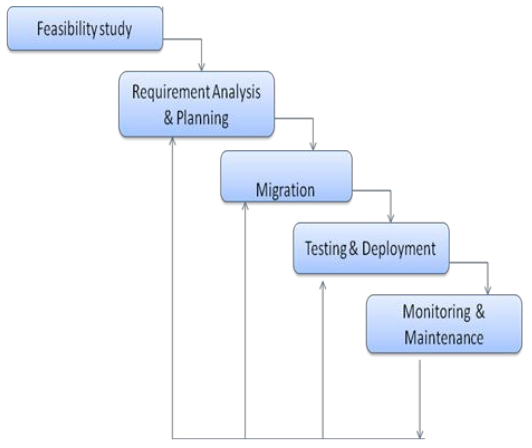
\includegraphics[width=0.6\textwidth]{images/fuenf-phasen-wasserfall-modell.png}
\caption{Das Fünf-Phasen-Wasserfallmodell aus \protect\citeflow{fivephases} }
\label{fuenf-phasen-wasserfall-modell}
\end{center}
\end{figure}
\begin{enumerate}
	\item Die technische und wirtschaftliche \textbf{Machbarkeitsstudie}
analysiert die bestehende Anwendung in Hinblick auf Dateneingabe, 
Datenverarbeitung, Datenausgabe und sonstige Randbedingungen und Erwartungen. 
Das Ergebnis der Machtbarkeitsstudie ist eine detaillierte  
Kosten-Nutzen-Analyse. Als Grundlage einer wirtschaftlich vernünftigen 
Migrationsentscheidung muss sie ergebnisoffen verlaufen.
	\item Die \textbf{Anforderungsanalyse und -Planung} konkretisiert die 
Ergebnisse der Machtbarkeitsstudie weiter, indem sie die oben genannten 
wirtschaftlichen und technischen Faktoren berücksichtigt. Außerdem wird der 
Return on Investment sowie die Total Cost of Ownership berechnet.
	\item Mit der \textbf{Migration} ist nicht nur die Entwicklung 
beziehungsweise Einrichtung der Cloudsoftware gemeint, sie enthält auch Tests 
der Funktionalität, Performanz und Nutzerakzeptanz.
	\item Beim \textbf{Ausrollen (Go-Live) und Testen} wird die 
Cloud-Anwendung mit den Betriebsdaten ausführlich getestet und 
schließlich freigegeben. Die Freigabe ist mit intensiver Beobachtung und 
verstärktem Support zu begleiten um auftretenden Problemen begegnen zu können. 
Je nach Größe, Relevanz und Art der Anwendung ist zu prüfen, ob in der 
Anfangsphase  ein paralleler Ansatz gewählt wird, bei dem die bestehende Lösung 
weiter genutzt wird.
	\item Naturgemäß ist man bei Nutzung der Cloud bei Performanz, 
Verfügbarkeit und Sicherheit vom Anbieter abhängig. Die Einhaltung garantierter 
Leistungen und Erwartungen sollte man \textbf{überwachen}. Abweichungen lassen 
sich Idealerweise  \textbf{Wartungsarbeiten} an der Anwendung oder durch 
Einforderung von Leistungen beim Anbieter beheben.
\end{enumerate}
\subsubsection{Organisationsform als Einflussfaktor}
\citeflow{fivephases} identifizieren die Organisationsstruktur, beziehungsweise 
deren Größe und Komplexität und insbesondere drei Formen als 
wesentliche Einflussfaktoren für dieses Vorgehensmodell. Zu diesem Ergebnis 
kommen auch \citeflow{Pahl2013}.
\begin{description}
	\item[Große Unternehmen] haben gewachsene, komplexe IT-Strukturen, die 
umso detailliertere Analysen der Cloud-Eignung einzelner Anwendungen 
erforderlich machen und eine Schrittweise Migration nahelegen, bei der 
zunächst einfache Standardanwendungen wie E-Mail-Anwendungen migriert werden. 
Komplexe Anwendungen folgen sobald Erfahrungen im Cloud-Umfeld gesammelt wurden 
und gegebenenfalls fertige Anwendungen in der Cloud bereits existieren.
	\item[Kleinere und mittlere Unternehmen] haben gegenüber großen 
Unternehmen nicht nur den Vorteil einer kleineren, weniger komplexen 
IT-Landschaft. Bestehende Unternehmensprozesse lassen sich auch leichter an die 
Cloud-Nutzung anpassen, sodass sich viele bereits in der Cloud existierende 
Cloud-Anwendungen als SaaS nutzen lassen. Durch die nutzungsabhängige 
Bepreisung lassen sich in der Cloud möglicherweise Anwendungen nutzen, die 
bisher zu teuer oder zu komplex waren. Die nutzungsabhängige Bezahlung birgt 
allerdings wie bereits geschildert auch Risiken, die neben den anderen Faktoren 
ebenfalls vor der Migrationsentscheidung berücksichtigt werden sollten.
	\item[Regierungsorganisationen] dürften regelmäßig zwei Spezifika 
aufweisen, die bei der Prüfung der Cloud-Eignung einer Anwendung zu prüfen 
sind. Erstens sind sie in besonderem Maße, teilweise durch Gesetze, zur 
Kontrolle über die eigenen Daten und Funktionsfähigkeit ihrer Anwendungen 
gezwungen. Zweitens übersteigt die orts-, amts- oder ministerienübergreifende 
Zusammenarbeit die Komplexität von großen Unternehmen bei weitem. 
\end{description}



\subsection{Methoden zur Anforderungsermittlung in Migrationsprojekten}
\subsection{Aktuelle und prognostizierte Ressourcennutzung}
\subsection{Auswahl des Migrationsziels in der Cloud}
\subsection{Kostenabschätzung der Cloud-Lösung}

\newpage
\subsection{Abbildungen}

\begin{figure}[h]
\begin{center}

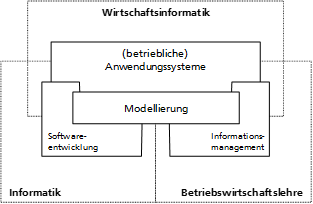
\includegraphics[width=10cm]{images/Abb2_3.png}
\caption{Einordnung der Wirtschaftsinformatik (angelehnt an Fink et al. 2001)}
\label{Abbildung2_3}
\end{center}
\end{figure}
Bitte achten Sie darauf, dass alle vorhandenen Abbildungen und Tabellen in einem inhaltlichen Zusammenhang mit dem Text stehen und Sie auf die entsprechende Abbildung (bspw. Abbildung 1) verweisen.
\subsection{Tabellen}
%hier Tabelle einfügen
\begin{table}[h]
\centering
\begin{tabular}{ccc}
\hline \textbf{Attribute} &\textbf{Typ}  & \textbf{1. Ausprägung (Beispiel)} \\ 
\hline Titel & \textit{STRING}& Aktiengesetz (AktG)  \\ 
Text& \textit{STRING} &  [Text des AktG]\\ 
Gültig von & \textit{DATE} & 01.01.2010 \\ 
Gültig bis & \textit{DATE} & - \\ 
Dok.-Besitzer & \textit{STRING} & Rechtsabteilung \\ 
Quelle & \textit{STRING}  & Deutsche Gesetze \\ 
Verplichtungsgrad & \textit{STRING} & verplichtend \\ 
\hline 
\end{tabular} 
\caption{Attribute der Anforderungsquellen im Metamodell}
\label{tab:tabelle 1}
\end{table}
\par\medskip

Tabelle 1 stellt eine beispielhafte Tabelle dar%2
%%\section{Entwicklung eines konzeptuellen Rahmens}
\section{Vorgehensmodell für Cloud-Migrationen zu Salesforce}
\label{cha:entwickelung_vorgehensmodell}
In diesem Kapitel soll das Fünf-Phasen-Modell angepasst und erweitert werden, 
um den Anforderungen eines Independent Software Vendors (ISV) zu entsprechen. \\

%\documentclass[border=10pt]{standalone}

\usetikzlibrary{decorations.text}
\usetikzlibrary{calc}
\usetikzlibrary{fit}
\usetikzlibrary{shapes}
\usetikzlibrary{arrows,positioning} 
\pgfmathsetmacro{\cubex}{4}
\pgfmathsetmacro{\cubey}{2}

\definecolor{light-gray}{gray}{0.80}

\tikzset{
    %Define standard arrow tip
    >=stealth',
    %Define style for boxes
    punkt/.style={
           rectangle,
           rounded corners,
           draw=black, very thick,
           text width=8em,
           minimum height=2em,
           text centered},
    % Define arrow style
    pil/.style={
           ->,
           very thick,
           shorten <=5pt,
           shorten >=5pt,},
    sepLine/.style={
	dashed,
	very thick
    }
}




%\begin{document}
\begin{figure}[bh]
\begin{center}
\scalebox{.8}{
\begin{tikzpicture}


\newcommand{\gear}[5]{%
    \foreach \i in {1,...,#1}
    {   [rotate=(\i-1)*360/#1] (0:#2) arc (0:#4:#2) {[rounded corners=0.5pt] -- 
(#4+#5:#3)  arc (#4+#5:360/#1-#5:#3)} --  (360/#1:#2)
    }
}      

% Punkte
\newcommand{\boxNO}{(0,0)}
\newcommand{\boxNW}{(-\cubex,0)}
\newcommand{\boxSO}{(0,-\cubey)}
\newcommand{\boxSW}{(-\cubex,-\cubey)}


% On-Premise-Produkt
\draw[black,fill=light-gray,very thick] \boxNW -- \boxNO -- \boxSO -- \boxSW -- 
cycle;
\draw (-0.5*\cubex,-0.5*\cubey) node {\textbf{On-Premise-Produkt}};

% Trichter
\newcommand{\trichterBreiteO}{1.5*\cubex}
\newcommand{\trichterBreiteM}{0.33*\cubex}
\newcommand{\trichterAbstand}{0.5*(\trichterBreite - \trichterBreiteM)}

\newcommand{\trX}{-1.25*\cubex}
\newcommand{\trY}{-1.25*\cubey}
\newcommand{\trichterNW}{ (\trX, \trY) }
\newcommand{\trichterNO}{ (\trX+\trichterBreiteO, \trY) }

\newcommand{\trichterMW}{ ( \trX + 0.33*\trichterBreiteO, \trY-0.75*\cubey ) }
\newcommand{\trichterMO}{ ( \trX + 0.66*\trichterBreiteO, \trY-0.75*\cubey ) }

\newcommand{\trichterSW}{ ( \trX + 0.33*\trichterBreiteO, \trY-1.75*\cubey) }
\newcommand{\trichterSO}{ ( \trX + 0.66*\trichterBreiteO, \trY-1.75*\cubey) }

\newcommand{\trichterC}{ ( \trX + 0.5*\trichterBreiteO, \trY-0.5*0.75*\cubey) }

\draw[black,thick] %,fill=SkyBlue 
	\trichterNW -- 
	\trichterNO -- 
	\trichterMO --
	\trichterSO --
	\trichterSW --
	\trichterMW --
	\trichterNW;
% Uncomment for text in Trichter
%\draw \trichterC node {};




% Diamond



\newcommand{\diamondX}{\trX + 0.5*\trichterBreiteO}
\newcommand{\diamondY}{\trY-2.4*\cubey}
%star point height=.9cm, minimum size=0.7*\cubey,draw,
\node [starburst, fill=Goldenrod,draw,starburst points=13] (VISION)
at (\diamondX,\diamondY) {Vision};
	
\newcommand{\boxREx}{\diamondX}
\newcommand{\boxREy}{\diamondY - 1.5*\cubey}
\newcommand{\boxRo}{1.8*\cubey}
\newcommand{\boxRm}{2*\cubey}
\newcommand{\boxRu}{1.2*\cubey}
\newcommand{\boxHEins}{.9*\cubey}
\newcommand{\boxHZwei}{2*\cubey}
\newcommand{\boxHDrei}{3*\cubey}


 \node[punkt] (RE) at (\boxREx,\boxREy) {Requirements Engineering} ;  
\node[punkt] (PL) at (\boxREx-\boxRo,\boxREy -\boxHEins)  {Planning}
 edge[pil] (RE.west) ;
 
 \node[punkt] (EVAL) at (\boxREx-\boxRm,\boxREy -\boxHZwei)  {Evaluation} 
edge[pil] (PL.south);
 
 
 \node[punkt] (T) at (\boxREx-\boxRu,\boxREy -\boxHDrei)  {Testing}
 edge[pil] (EVAL.south) ;
 
 
 \node[punkt] (DEPL) at (\boxREx+\boxRu,\boxREy -\boxHDrei)  {Deployment}
 edge[pil] (T.east);
 
 
 \node[punkt] (I) at (\boxREx+\boxRm,\boxREy -\boxHZwei)  {Implementation}
 edge[pil] (DEPL.north);
 
 \node[punkt] (AD) at (\boxREx+\boxRo,\boxREy -\boxHEins)  {Analysis \& Design}
edge[pil] (I.north);

\draw[pil]
  (RE.east) edge (AD.north);
  
% Pfeil+Text Vision -> RE
\draw[pil] (VISION) edge (RE.north);% {Wie sieht es hier aus?};

%\node (UMSETZBARKEIT) at (\diamondX+0.25*\cubex,\diamondY-0.6*\cubey) 
%{\Large{1001 ?}};
 %(formidler) {Intermediaries (c)};
 
% given
\pgfmathsetmacro{\rOne}{0.2}% inner radius
\pgfmathsetmacro{\nOne}{11}% num teeth
\pgfmathsetmacro{\nTwo}{15}
\pgfmathsetmacro{\nThree}{19}
\pgfmathsetmacro{\toothHeight}{0.4*\rOne}
\pgfmathsetmacro{\toothFall}{1}% degrees where radius drops from inner 
to %outer
\pgfmathsetmacro{\aOneTwo}{120}% angle from first to second
\pgfmathsetmacro{\aTwoThree}{40}% angle from first to second

% computed
\pgfmathsetmacro{\rTwo}{\rOne*\nTwo/\nOne}% via equating tooth lengths
\pgfmathsetmacro{\rThree}{\rOne*\nThree/\nOne}% 
\pgfmathsetmacro{\ROne}{\rOne+\toothHeight}% outer radius
\pgfmathsetmacro{\RTwo}{\rTwo+\toothHeight}
\pgfmathsetmacro{\RThree}{\rThree+\toothHeight}
\pgfmathsetmacro{\dOne}{(360/\nOne-\toothFall)/2}% degrees for a tooth; here 
inner deg = outer deg
\pgfmathsetmacro{\dTwo}{(360/\nTwo-\toothFall)/2}
\pgfmathsetmacro{\dThree}{(360/\nThree-\toothFall)/2}
\pgfmathsetmacro{\distOneTwo}{\rOne+\rTwo+\toothHeight+0.05}
\pgfmathsetmacro{\distTwoThree}{\rTwo+\rThree+\toothHeight+0.05}

\coordinate (A) at (\diamondX+0.5*\cubex,\diamondY-0.8*\cubey);
\coordinate (B) at ($(A)+(\aOneTwo:\distOneTwo)$);
\coordinate (C) at ($(B)+(\aTwoThree:\distTwoThree)$);  

\draw[thick, rotate=10] node[align=center] {} ;
%\gear{\nOne}{\rOne}{\ROne}{\dOne}{\toothFall} ;

\draw[thick, shift={(B)}, rotate=18] node[align=center] {} 
\gear{\nTwo}{\rTwo}{\RTwo}{\dTwo}{\toothFall};
\draw[thick, shift={(C)}, rotate=8] node[align=center] {} 
\gear{\nThree}{\rThree}{\RThree}{\dThree}{\toothFall};

\node[scale=1.5] (TECHQ) at ($ (A) + (0.3*\cubex,0.4*\cubey) $) {\Huge{?}};
\node[scale=1.5] (WIRTQ) at (\diamondX-0.6*\cubex,\diamondY-0.4*\cubey) 
{\Huge{€?}};
 
% Cloud 
\node [cloud, draw,cloud puffs=10,cloud puff arc=120, aspect=2, inner 
ysep=3*\cubex,fill=Goldenrod] (CLOUD) at (\boxREx,\boxREy-0.8*\boxHZwei) 
{\textbf{Cloud L\"osung}};
 
% Linien
\newcommand{\firstLineY}{\trY - 1.9 * \cubey}
\draw[sepLine] (\trX-\boxRm, \firstLineY) -- (\trX + 2.3*\boxRm, 
\firstLineY);

\newcommand{\secondLineY}{\diamondY - .85 * \cubey}
\draw[sepLine] (\trX-\boxRm, \secondLineY) -- (\trX + 2.3*\boxRm, 
\secondLineY);

% Phasen
\newcommand{\circlesX}{\diamondX-1.5*\boxRm}
\draw (\circlesX,\diamondY + 1.2*\cubey) circle [radius=0.4*\cubey] node 
{\Huge{I}};
\draw (\circlesX,\diamondY - 0.2*\cubey) circle [radius=0.4*\cubey] node 
{\Huge{II}};
\draw (\circlesX,\diamondY - 1.5*\cubey) circle [radius=0.4*\cubey] node 
{\Huge{III}};
 
 %\node[punkt, inner sep=5pt,below=0.5cm of RE]
 %(formidler) {Intermediaries (c)};
 % We make a dummy figure to make everything look nice.
 %\node[above=of RE] (dummy) {};
 %\node[right=of dummy] (t) {Ultimate borrower}
  %edge[pil,bend left=45] (RE.east) % edges are used to connect two nodes
  % edge[pil, bend left=45] (I.east); % .east since we want
                                             % consistent style
 %\node[left=of dummy] (g) {Ultimate lender}
   %edge[pil, bend right=45] (RE.west)
   %edge[pil,<->, bend left=45] node[auto] {Direct (a)} (t);
	
\end{tikzpicture}
}
\caption{Darstellung des Vorgehensmodells. Der iterative Software Engineering 
Kreislauf wurde \cite{changes_in_requirements_engineering} entnommen.}
\label{fig:vorgehensmodell}
\end{center}
\end{figure}

%\end{document}





Das Fünf-Phasen-Modell beginnt mit einer technischen und 
wirtschaftlichen Machbarkeitsstudie. Die Migration einer On-Premise-Software in 
die Cloud bedeutet für das migrierende Unternehmen die Erschließung eines ganz 
neuen Marktes, der sich grundlegend vom bekannten Markt unterscheidet. Aus 
diesem Grund kann das Cloud-Produkt sich grundlegend vom bisherigen 
On-Premise-Produkt unterscheiden. Deshalb wird 
\citeflow{how_saas_changes_an_isvs_business} und 
\citeflow{towards_modelling_a_cloud_applications_life_cycle} eine zusätzliche 
Phase vorgeschlagen, in der eine Vision der künftigen Cloud-Lösung entworfen 
wird. Mit dieser Vision kann der Leistungsumfang abgeschätzt werden und auch, 
wie sich das Unternehmen verändern muss, um dieser Vision zu entsprechen. 
(Kapitel~\ref{cha:phaseI})\\

Anschließend kann in Phase II... \\

In Phase III... \\

In Phase IV... \\

In Phase V... \\

In Phase VI... \\

\subsection{Phase I: Entwicklung einer Vision}
\label{cha:phaseI}

Als "`disruptive innovation"' ist die Cloud auch ein neuer Markt, auf dem 
qualitativ hochwertige, teilweise hoch spezialisierte IT-Dienstleistungen 
gehandelt werden. 
\pcite{}{}{towards_modelling_a_cloud_applications_life_cycle} \\
Durch das pay-per-use-Preismodell sind auch kleine Unternehmen in der Lage, 
diese Technologien und Dienstleistungen zu nutzen. 
\pcite{}{156}{cloud_migration} Dementsprechend ist die Nutzung der Cloud per se 
weder  innovativ -- da jeder Mitbewerber die Technologie nutzen kann -- noch 
ein Wettbewerbsvorteil: Sie ist ein wirtschaftliches Erfordernis, um den 
Wettbewerb nicht zu verlieren. 
\pcite{}{}{challenges_of_cloud_computing_in_business} 


Damit die in die Cloud migrierte Software dem Unternehmen auch einen anhaltenden 
Wettbewerbsvorteil bieten kann, muss sie einen Wert für den Kunden schaffen, 
unter aktuellen und möglichen zukünftigen Konkurrenten einzigartig oder 
wenigstens selten sein, annähernd unnachahmlich und schwer substituierbar sein.
\pcite{}{}{theoretical_perspectives_for_strategic_human_resource_management} 
\begin{comment}
zufolge
\begin{itemize}
  \item dem Unternehmen einen positiven Wert hinzufügen
  \item unter aktuellen oder möglichen zukünftigen Konkurrenten einzigartig oder 
selten sein
  \item annähernd unnachahmlich
  \item durch Konkurrenten schwer substituierbar sein
\end{itemize}
\end{comment}
Um diesen Anforderungen gerecht zu werden, bedarf es einer geschickten 
Integration standardisierter, in der Cloud verfügbaren Komponenten zu einer 
innovativen Gesamtlösung. Gelingt dies nicht, ist eine Differenzierung von 
konkurrierenden, sich gleichenden Produkten nur über einen niedrigeren Preis 
möglich. \pcite{}{}{towards_modelling_a_cloud_applications_life_cycle} \\

Diese Anforderungen berücksichtigend, sollen -- angelehnt an die Methode der 
SWOT-Analyse \pcite{}{501}{marketingmanagement} -- Chancen und Risiken der 
Cloud betrachtet werden und schließlich in eine Vision. \\

Auch wenn in diesem Modell, als Ergebnis dieser Phase nur die Vision des 
Produktes in den folgenden Phasen weiter verfolgt wird, sollten Chancen und 
Risiken -- ob technischer oder wirtschaftlicher Natur -- auch in Hinblick auf 
ihre Auswirkungen auf das Geschäftsmodell und die 
Unternehmensorganisation des ISV hin untersucht werden. \\

\subsubsection{Geschäftsmodell}
Aus einer technologischen Innovation wird für ein Unternehmen erst ein Wert, 
wenn es mit einem erfolgreichen Geschäftsmodell vermarktet werden kann. Gerade 
beim Auftreten von "`disruptives innovations"' scheitern viele Unternehmen, 
weil sie nicht in der Lage oder willens sind, ihr Geschäftsmodell in 
ausreichendem Maße zu 
ändern. \pcite{}{}{disruptive_technologies_a_business_model_perspective} Um ein 
wirtschaftlich nachhaltiges, an die Realitäten des Marktes angepasstes, 
wettbewerbsfähiges Geschäftsmodell für den Cloud-Markt zu entwickeln, sollte 
der ISV unter Berücksichtigung der Chancen und Risiken die folgenden Fragen 
beantworten \citeflow{disruptive_technologies_a_business_model_perspective}:
\begin{enumerate}
	\item Wie entsteht für den Kunden Wert in Form eines Produktes oder 
		einer Dienstleistung?
	\item In welcher Form und Höhe und mit welchem Preismodell wird Umsatz 
generiert? 
	\item Wie können bereits bestehende und kommende standardisierte 
Komponenten und Dienstleistungen in das Produkt integriert werden?
	\item Wie lassen sich bestehende oder zu erwerbende Ressourcen und 
Fähigkeiten (andersartig) nutzen, um neue Produkte oder Dienstleistungen zu 
erzeugen?
	\item Mit welchen strategischen Entscheidungen lassen sich 
Wettbewerbsvorteile (auch gegenüber On-Premise-Lösungen und 
zugehörigen Preismodellen) erlangen?
\end{enumerate}

\begin{comment}
\subsubsection{Organisationsstruktur}
Da der Kunde des ISV keine Serverinfrastruktur betreiben muss, um die 
Cloud-Lösung zu nutzen und auch auf den Rechnern der Endbenutzer nichts 
installiert werden muss, entfallen im Idealfall Verhandlungen zwischen ISV und 
der IT-Abteilung des Kunden; Entscheidungen werden in kleineren Kreisen, direkt 
von Fachabteilungen getroffen. Für den ISV hat dies zur Folge, dass er mit 

Als Abstraktionsschicht ermöglicht es Cloud-Computing Unternehmen die 
Wertschöpfungskette zu verschlanken und sich auf ihr Kerngeschäft zu 
konzentrieren.

Cloud-Computing wird im Ideal als Abstraktionsschicht gesehen, die 
Komplexitäten 
vor Fachabteilungen und Führungskräften verbirgt und es ihnen ermöglicht ohne 
Entwickler. Wo in der Vergangenheit Empfehlungen, Design, Entwicklung, 
Deployment und Wartung in den Händen von IT-Abteilungen lagen, ist es im 
Cloud-Computing nötig, dass Führungskräfte

Auf dem Weg zum einzigartigen, innovativen und wettbewerbsfähigen Produkt, muss 
sich ein Unternehmen auf seine Kernkompetenzen konzentrieren und 
das Thema IT neu betrachten, um die Flexibilität und Agilität der Cloud nutzen 
zu können. Anstatt sich in der Hauptsache die bestehende 
IT-Infrastruktur zu unterhalten, werden IT-Abteilungen zu strategischen 
Partnern 
in der Weiterentwicklung der Produkte 
\pcite{}{}{how_saas_changes_an_isvs_business}: Mitarbeiter aus der IT müssen 
genutzt werden, um qualitativ hochwertige, nutzbare 
Trends bei Cloud-Dienstleistungen frühzeitig zu erkennen und kreativ in das 
Produkt einfließen zu lassen oder Business-Prozesse bestmöglich zu 
unterstützen.
\end{comment}


\subsubsection{Chancen \& Risiken der Cloud-Migration}
\label{cha:chancen_und_risken}
Chancen und Risiken einer Cloud-Migration für einen Independent Software 
Vendor sind Ergebnis der Literaturrecherche und finden sich in den
Tabellen~\ref{tab:chancen_der_cloud} und \ref{tab:risiken_der_cloud}. Die 
Spalte "`Fragen \& Aufgaben für den ISV"' soll dabei helfen, eine 
Produktvision zu entwickeln, die dem Unternehmen einen anhaltenden 
Wettbewerbsvorteil bescheren soll.


\newcommand{\cloudFeature}[4]{
\item[#1] \hfill \\
\textbf{Beschreibung:} #2 \\
\textbf{Quelle(n):} \pcite{}{}{#3} \\
\textbf{Fragen \& Herausforderungen:} #4
}

\begin{description}
	\cloudFeature{Soziales Element}
	{Das soziale Element entsteht durch neue Möglichkeiten 
des Austausches, die durch die Nutzung einer gemeinsamen Cloud-Plattform 
entstehen: zwischen Nutzern innerhalb eines Unternehmens, zwischen 
verschiedenen Unternehmen oder mit den Entwicklern. Die Weiterentwicklung wird 
dadurch inklusiver, Nutzer lassen sich einbeziehen.}
	{cloud_based_next_generation_service_and_key_challenges, 
changes_in_requirements_engineering}
	{Wie lässt sich der Kontakt zu und zwischen Kunden und ihren 
Fachabteilungen so 
direkt, einfach und produktiv wie möglich gestalten? Lassen sich Communities 
aufbauen?}

	\cloudFeature{Analysemöglichkeiten}{Da sich alle Benutzer auf der Cloud 
bewegen, fallen viel mehr Informationen an, die analysiert werden 
können}{cloud_based_next_generation_service_and_key_challenges,
changes_in_requirements_engineering}{Wie lassen 
sich künftige Entscheidungen mit den gewonnenen Informationen fundierter 
treffen?}

\cloudFeature{Mobilität }{ Lösungen aus SaaS-Bereich sind häufig bereits im 
Standard auf 
mobile Bedienbarkeit 
ausgelegt. }{cloud_based_next_generation_service_and_key_challenges} { 
Um bezüglich Mobilität nicht nur Erwartungen zu erfüllen, sondern 
Begeisterung zu wecken, sollte geprüft werden, wie die gewonnene Mobilität im 
konkreten Fall den Kundenwert steigern kann. }
%%%%%%%%%%%%%%%%%%%%%%%%%%%%%%%%%%%%%%%%%%%%%%%%%%%%%%%%%%%%%%%%%

\cloudFeature{Reduzierte Markteintrittskosten, Skalierte Märkte }{ Durch 
pay-per-use-Modelle 
sind die Markteintrittskosten drastisch reduziert.
}{cloud-computing_the_business_perspective} { Mit welchen Produkten 
lassen sich neue Märkte erschließen? Welche unerschlossenen Märkte gibt es? Wie 
lassen sich geographisch weit entfernte Märkte erschließen? }

%%%%%%%%%%%%%%%%%%%%%%%%%%%%%%%%%%%%%%%%%%%%%%%%%%%%%%%%%%%%%%%%%
\cloudFeature{Skalierung der Leistung }{ In der Cloud stehen -- dynamisch an den 
aktuellen 
Bedarf angepasst -- unbegrenzte Ressourcen bereit.
}{cloud-computing_the_business_perspective} { Wie lassen sich die 
Ressourcen nutzen, um gegenüber On-Premise-Anwendungen im Vorteil zu sein? }
%%%%%%%%%%%%%%%%%%%%%%%%%%%%%%%%%%%%%%%%%%%%%%%%%%%%%%%%%%%%%%%%%

\cloudFeature{Time to market, kürzere Releasezyklen }{ 
Die Software und auch Updates lassen sich schneller auf den Markt bringen. 
}{changes_in_requirements_engineering,
towards_an_understanding_of_cloud_computings_impact_on_org_it_strategy}{}

\cloudFeature{Alternativen testen }{ 
In der Cloud lassen sich alternative Implementierungen 
testen und direkt auswerten.}{changes_in_requirements_engineering} {} 

\cloudFeature{Sparen der Wartung älterer Versionen }{ 
Kapazitäten werden frei, da es in der Cloud nur eine aktuelle Version gibt, in 
die alle Entwicklungsarbeit fließen kann und keine Altversionen gewartet und 
berücksichtigt werden müssen. 
}{changes_in_requirements_engineering,transitioning_to_saas} {}

\cloudFeature{Standardisierte Komponenten}{Mit in der Cloud verfügbaren, 
standardisierten Komponenten lassen und loser Kopplung lassen sich 
Funktionen relativ leicht 
ergänzen}
{towards_an_understanding_of_cloud_computings_impact_on_org_it_strategy,
cloud_based_next_generation_service_and_key_challenges}{}
\end{description}


\begin{table}[ht!]
\centering
\begin{longtable}{|p{0.11\textwidth}|p{0.4\textwidth}|p{0.4\textwidth}|}
\hline
\textbf{Stichwort} & \textbf{Beschreibung \& Quelle} & \textbf{Fragen \& 
Aufgaben für den ISV} \\
\hline %%%%%%%%%%%%%%%%%%%%%%%%%%%%%%%%%%%%%%%%%%%%%%%%%%%%%%%%%%%%%%%%%

\hline %%%%%%%%%%%%%%%%%%%%%%%%%%%%%%%%%%%%%%%%%%%%%%%%%%%%%%%%%%%%%%%%%
\end{longtable}
\caption{Mögliche Risiken durch die Migration in die Cloud}
\label{tab:risiken_der_cloud}
\end{table}

\subsubsection{Produktvision}
\citeflow{fivephases} schlagen ihr Fünf-Phasen-Modell für eine vollständige 
Migration einer Software und der Gesamtheit ihrer Funktionalität vor. Von 
dieser Vorgabe wird in dem hier vorgestellten Modell aus zweierlei Gründen 
abgewichen. \\
Erstens wird es mit einer 1:1-Migration weder möglich sein die in 
Kapitel~\ref{cha:chancen_und_risken} genannten Vorteile zu realisieren, noch 
die Risiken zu umschiffen. \\
Eine vollständige Migration und eine erst daran anschließende Vermarktung würde 
viel Zeit in Anspruch nehmen, in der keine Umsätze generiert werden. Dadurch 
steigt zweitens das finanzielle Risiko und das Unternehmen läuft Gefahr das 
gesetzte Cloud-Ziel von mehr Flexibilität, höherer Agilität und schnellere 
Innovationsgeschwindigkeit zu verfehlen. Denn dabei würde ein Vorteil der 
Cloud vollkommen ignoriert: Die Software lässt sich leicht aktualisieren, 
während der Kunde bereits mit ihr arbeitet. Dies ermöglicht eine Agilität, wie 
sie nicht möglich ist, wenn Software erst ausgeliefert und vom Kunde installiert 
werden muss. Es wäre denkbar, dass Erfahrungen des Kunden im Umgang mit dem 
jeweils aktuellen Stand der Software in die Sprint-Planung eingehen. Die 
Weiterentwicklung der Software wäre damit eng an die tatsächlichen Bedürfnisse 
der Kunden gekoppelt. \\

Aus den genannten Gründen wird in dieser Arbeit sprintweise Migration und 
Weiterentwicklung vorgeschlagen, die mit einer Produktvision beginnt. 
Abgeleitet aus den Eigenschaften, die Unternehmensvisionen laut 
\citeflow{the_power_of_vision} aufweisen sollten, werden die folgenden Merkmale 
für eine Produktvision vorgeschlagen:
\begin{itemize}
	\item Sie sollte die genannten Chancen und Risiken berücksichtigen.
	\item Der Umfang des Produktes sollte so klein wie möglich, so 
umfangreich wie nötig sein, um frühestmöglich einen auslieferbaren Wert zu 
schaffen. 
	\item Die Architektur sollte -- in Hinblick auf zusätzliche 
Cloud-Komponenten, Dienstleistungen und das Datenmodell -- erweiterbar sein.
\end{itemize} 

Aus \citeflow{the_power_of_vision}:
\begin{itemize}
	\item Vision ist strategische Überlegung um wettbewerbsfähiges Produkt 
zu schaffen
	\item Unterscheidung nötig zwischen starken und schwachen Visionen, 
positiven und negativen
	\item Eigenschaften guter Visionen: \\
	\begin{itemize}
		\item conciseness - kurz
		\item clarity - prime goal, easy (in 5 minutes) to understand
		\item future orientation - long term
		\item stability - Vision reagiert nicht auf kurzfristige Trends
		\item challenge - high but achievable difficulty
		\item abstractness
		\item desirability or ability to inspire
	\end{itemize}
	\item Notwendigkeiten um Vision zu realisieren: \\
	\begin{itemize}
		\item communicating the vision
		\item aligning organizational processes and systems to suit the 
vision
		\item empowering others to act to achieve the vision
		\item motivating staff
	\end{itemize}
	\item Charakterisitika eng mit Unternehmenserfolg verbunden


\end{itemize}

\subsubsection{TODO: Preismodell, frühe Vermarktung eines Produktes mit 
geringerem Umfang}

\begin{comment}

\subsection{Phase I: Business, Strategie und Struktur neu gestalten}

\subsubsection{IT-Strategie}
Unter einer IT-Strategie 
verstehen \citeflow{
towards_an_understanding_of_cloud_computings_impact_on_org_it_strategy} die 
organisationsweite Perspektive auf Investitionen in IT-Systeme sowie das 
Deployment, die Nutzung und das Management von IT-Systemen. Die IT-Strategie 
legt insbesondere fest
\begin{itemize}
	\item welchen Umfang die IT im Unternehmen hat
	\item welche IT-Fähigkeiten vorgehalten werden
	\item wie Steuerung und Controlling erfolgen
	\item wie das Anwendungsportfolio zusammengestellt ist
	\item wie Daten verarbeitet und gespeichert werden
	\item wie IT und Business aufeinander abgestimmt werden
\end{itemize}
\citeflow{
towards_an_understanding_of_cloud_computings_impact_on_org_it_strategy} 
identifizieren einige Auswirkungen einer Cloud-Migrationen auf die IT-Strategie 
für Unternehmen. Aus den allgemein gehaltenen Auswirkungen, werden Vorschläge 
abgeleitet, die sich an Independent Software Vendors richtet.
\begin{description}
  \item[Architektur] Bei klassischen On-Premise-Anwendung war es in der Regel 
nötig, Änderungen äußerst sorgfältig und langfristig zu planen, da sich Fehler 
aufgrund monolithischer Architekturen auf das gesamte System ausgewirkt hätten. 
Die geringe Geschwindigkeit verhindert schnelle Release-Zyklen von 
wenigen Wochen, die in der Cloud erwartet werden. In der Cloud lassen sich neue 
Funktionalitäten durch die lose Kopplung vorgefertigter Komponenten ergänzen. 
\pcite{}{}{cloud_based_next_generation_service_and_key_challenges} Da die 
Komplexität mit zunehmender Zahl von Komponenten -- gerade von verschiedenen 
Anbietern -- trotzdem zunimmt, sollten zukünftige Anforderungen bedacht werden.
  \item[Datenverarbeitung und -Speicherung] Der ISV sollte frühzeitig bedenken, 
welche Daten seiner Kunden in welchem Umfang auf welche Weise in die Cloud 
migriert werden müssen. Inkonsistenzen in den Daten, die auftreten können, wenn 
Daten inkrementell übertragen werden müssen, die Übertragung zeitintensiv ist 
oder wenn On-Premise- und Cloud-Lösung zunächst parallel betrieben werden, 
sind zu berücksichtigen. \\
\end{description}









\begin{comment}
Hauptmotivation die Cloud zu Nutzen, sollte nicht die Reduktion von Kosten
sein, sondern strategische Vorteile, wie eine Konzentration auf das
Kerngeschäft, schnellere und effizientere Innovationsprozesse,
Produktivitätssteigerungen und eine IT, die das Business besser unterstützt,
womöglich sogar profitabel ist. \pcite{}{}{the_strategic_value_of_the_cloud}

Gerade weil die Migration in die Cloud große technische aber vor allem auch
geschäftliche Umwälzungen mit sich bringt, sollte die Migration wirtschaftlich
begründet werden, genauer gesagt:
strategisch. \pcite{}{}{challenges_and_assessment_in_migrating} Auch wenn die
Nutzung der Cloud Einsparungen ermöglicht, machen IT-Budgets in der Regel
nur einen geringen Prozentsatz des Umsatzes aus. Hauptmotivation für die
Migration in die Cloud sollten deshalb strategische Ziele sein, mit denen der
Umsatz ausgebaut oder zumindest behauptet wer
\end{comment}

\begin{comment}
\subsubsection{SWOT-Analyse}
Aus \pcite{}{}{cloud-computing_the_business_perspective}
\begin{description}
	\item[Strengths] \hfill \\
	\begin{itemize}
		\item Skalierbarkeit
		\item 
	\end{itemize}
	\item[Weaknesses] \hfill \\
	\item[Opportunities] \hfill \\
	\item[Threats] \hfill \\
	
\end{description}
\end{comment}



\subsection{Phase II: Machbarkeitsstudie}
Phase II entspricht weitgehend der ersten Phase aus \citeflow{fivephases}: 
Durchführung einer technischen und wirtschaftlichen Machbarkeitsstudie. Objekt 
der beiden Machbarkeitsstudien ist hier jedoch die Produktvision, nicht die 
On-Premise-Software.\\
Dies wirkt sich vor allem auf die Prüfung der Wirtschaftlichkeit aus. Der 
Vorschlag des Fünf-Phasen-Modells an dieser Stelle eine "`detaillierte 
Kosten-Nutzen-Analyse"' durchzuführen, wird hier nicht 
befolgt. Um diese Entscheidung zu begründen, sollen die beiden 
Migrationsansätze noch einmal verglichen werden.\\
\usetikzlibrary{arrows}
\begin{figure}[bh]

\begin{center}

\scalebox{.8}{
\begin{tikzpicture}
\newcommand{\rechts}{6}
\newcommand{\radius}{1.9cm}
\coordinate (centerTop) at (\rechts,3.5);
\coordinate (centerLinks) at (0,0);
\coordinate (centerRechts) at (\rechts,0);
\coordinate (centerBottom) at (\rechts,-1);

% Linker Kreis
\draw (centerLinks) circle (\radius) node [text=black] 
{On-Premise-Lösung};


% Oberer Kreis
\draw[fill=green] (centerTop) circle (\radius);
\node[align=left] at ($ (centerTop) + (3.5,0)$) {Chancen};

%Unterer Kreis mit Schrift
\draw[fill=red] (centerBottom) circle (\radius);
\node[align=left] at ($ (centerBottom) + (3.5,-1)$) {Risiken};


% Rechte Mitte
\draw (centerRechts) circle (\radius);
\node[align=left] at ($ (centerRechts) + (3.5,0)$) 
{\st{On-Premise-}\\Cloud-Lösung};

% Pfeil
\path[draw=black,solid,line width=1mm,fill=black,
preaction={-triangle 90,thin,draw,shorten >=-1mm}
] ($ (centerLinks) + (1.2 * \radius,0) $) -- ($ (centerRechts) + 
(-1.2 * \radius,0) $);

%\draw \secondcircle node [text=black,left] {On-Premise-Software};
%\draw \thirdcircle node [text=black,right] {$C$};
\end{tikzpicture}
}
\caption{Funktionsumfang vor und nach der Migration im Wasserfallmodell. 
Selbsterstellte Grafik.}
\label{fig:funktionsumfang_wasserfallmodell}
\end{center}
\end{figure}

In Abbildung~\ref{fig:funktionsumfang_wasserfallmodell} ist der Ansatz aus dem 
Fünf-Phasen-Modell dargestellt. Dabei wird die bestehende Anwendung in ihrem 
gesamten Umfang in die PaaS/SaaS-Cloud migriert und erst daran anschließend 
vermarktet. Zumindest die Chance, eine agile Cloud-Lösung zu schaffen, die 
bereits früh einen Wert für Kunden schafft und sich schnell und an 
Kundenwünschen orientiert weiterentwickelt, wird verschenkt. Der ISV 
läuft aber auch Gefahr weitere Vorteile nicht zu realisieren, wenn er bei der 
Migration zunächst die Herstellung aller Funktionalitäten der Altsoftware in 
den Vordergrund stellt und dabei vernachlässigt, über Möglichkeiten 
nachzudenken, die Vorteile und Chancen der Cloud umzusetzen. Deshalb hat die 
Menge der Chancen nur zu einem geringen Teil in der Cloud-Lösung enthalten -- 
im Gegensatz zu den Risiken, die Teil der Cloud-Lösung werden, wenn man sich 
ihrer nicht bewusst ist und sie daher nicht vermeiden kann. \\
Abbildung~\ref{fig:funktionsumfang_agil} zeigt die in dieser Arbeit 
vorgeschlagene Vorgehensweise. Hier ist die Cloud-Lösung in ihrem Umfang sehr 
viel kleiner als die bestehende On-Premise-Software, sodass sie gerade das 
enthält, was für die Vermarktung nötig ist. Die Beschränkung des Umfangs 
begünstigt eine schnelle Fertigstellung und Vermarktung. Fehlendes Features 
werden agil nachentwickelt und in kurzen Abständen freigegeben. In der 
Cloud-Lösung werden von Anfang an Chancen und Risiken berücksichtigt und 
maximiert beziehungsweise minimiert. \\

Im Ergebnis ist das hier vorgestellte Vorgehen weniger riskant, da nötige 
Investitionen geringer sind und Fehler wie Erfolge schneller sichtbar werden. 
Da in diesem Modell zudem nicht die Kosteneinsparungen sondern strategische 
Ziele im Vordergrund stehen und der zeitliche Horizont viel kleiner ist, kann 
die Wirtschaftlichkeitsprüfung weniger detailliert ausfallen. Es sollte geprüft 
geprüft werden, ob nötige Umsätze mit dem Funktionsumfang der Vision generiert 
werden können. \\

\usetikzlibrary{arrows}
\begin{figure}[h]
\begin{center}

\scalebox{.8}{
\begin{tikzpicture}
\newcommand{\rechts}{6}
\newcommand{\radius}{1.9cm}
\coordinate (centerTop) at (\rechts,1.2);
\coordinate (centerLinks) at (0,0);
\coordinate (centerRechts) at (\rechts,0);
\coordinate (centerBottom) at (\rechts,-3.2);

% Linker Kreis
\draw (centerLinks) circle (1.5*\radius) node [text=black] 
{On-Premise-Lösung};


% Oberer Kreis
\draw[fill=green] (centerTop) circle (\radius);
\node[align=left] at ($ (centerTop) + (3.5,1)$) {Chancen};

%Unterer Kreis mit Schrift
\draw[fill=red] (centerBottom) circle (\radius);
\node[align=left] at ($ (centerBottom) + (3.5,0)$) {Risiken};


% Rechte Mitte
\draw (centerRechts) circle (0.8*\radius);
\node[align=left] at ($ (centerRechts) + (3.5,0)$) {Cloud-Lösung};

% Pfeil
\path[draw=black,solid,line width=1mm,fill=black,
preaction={-triangle 90,thin,draw,shorten >=-1mm}
] ($ (centerLinks) + (1.6 * \radius,0) $) -- ($ (centerRechts) + 
(-1.1 * \radius,0) $);

%\draw \secondcircle node [text=black,left] {On-Premise-Software};
%\draw \thirdcircle node [text=black,right] {$C$};
\end{tikzpicture}
}
\caption{Funktionsumfang vor und nach der Migration nach dem in dieser Arbeit 
vorgestellten Vorgehensweise. 
Selbsterstellte Grafik.}
\label{fig:funktionsumfang_agil}
\end{center}
\end{figure}



\begin{comment}
\subsubsection{Technische Machbarkeit}


\subsubsection{Wirtschaftliche Machbarkeit}
"`In diesem Punkt unterscheidet sich Cloud-Computing von früheren Paradigmen
wie Outsourcing, welches nicht auf das Geschäftsmodell des Unternehmens wirken
will. Durch neue Anwendungsszenarien kann mit Cloud-Computing ein beachtlicher
Mehrwert geschaffen werden."' \pcite{}{154}{cloud_migration}

"`Cloud-Computing verändert die Preisgestaltung von IT-Services und kann als
eine Reaktion  auf das straffere Kostenmanagement im Nachgang der Finanzkrise
2008 verwendet werden. Unternehmenskunden wollen sich nicht mehr mit fixen
IT-Kosten binden. Sie wollen auch in der IT des Unternehmens die Capital
Expenditures (CAPEX) in Operational Expenditures (OPEX) umwandeln. Dies ist der
Hauptgrund, wieso das 'Pay-per-Use-Pricing' von Cloud-Services bei den
 Unternehmen so viel Interesse geweckt hat."' \pcite{}{156}{cloud_migration}


"`Mögliche betriebswirtschaftliche Vorteile: bessere Nutzung des
Ressourcen-Pools des Unternehmens, Verbesserung der Zeit zur Markteinführung
neuer Produkte und Dienstleistungen, Steigerung der Agilität und letztlich
Verbesserung der Erfahrungen der Kunden im Umgang mit dem Unternehmen,
welches auf Cloud-Computing setzt."'
\pcite{}{157}{cloud_migration}


"`Alle Empfehlungen sollten mit einem Business Case hinterlegt werden, der
die Höhe der Kostenreduktion und die Verbesserung des Servicelevels zeigt."'
\pcite{}{158}{cloud_migration}
\end{comment}


\subsection{Phase III: Anforderungsanalyse und -Planung}
Der Software Engineering Prozess bei der Migration zu einem 
Software-as-a-Service-Modell ändert sich. 
\citepara{changes_in_requirements_engineering}

Anforderungsermittlung oder Requirementsengineering hat das Ziel Anforderungen 
eines Softwaresystem oder eines Features zu erheben, zu strukturieren, 
priorisieren und zu koordinieren. 
\pcite{}{}{changes_in_requirements_engineering} Auch die Identifizierung von 
Indiskrepanzen zwischen Ergebnis und Ziel gehört dazu. 
\pcite{}{}{requirements_engineering_process_for_saas_cloud_env}

Die Migration in die Cloud macht ein Überdenken der Software Engineering 
Prozesse notwendig. \pcite{}{}{transitioning_to_saas}

Besseres Requirements Engineering kann Kosten für die Fehlbehebung um 20\% 
senken.

\begin{figure}[!h]
\begin{center}
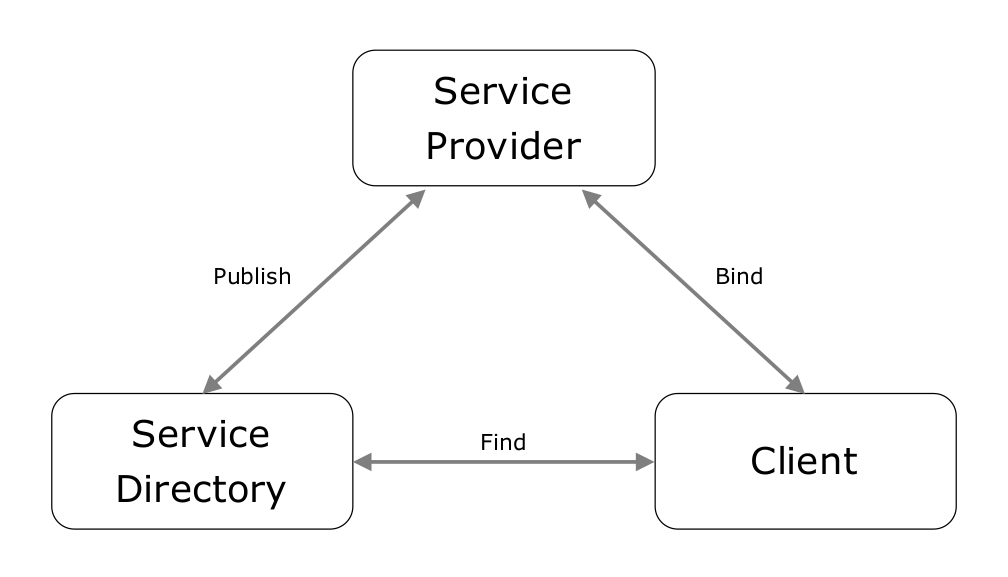
\includegraphics[width=0.8\textwidth]{images/soa_architecture.png}
\caption{Service-oriented architecture. Aus 
\protect\citeflow{changes_in_requirements_engineering}}
\label{fig:soa_architecture}
\end{center}
\end{figure}

\begin{figure}[!h]
\begin{center}
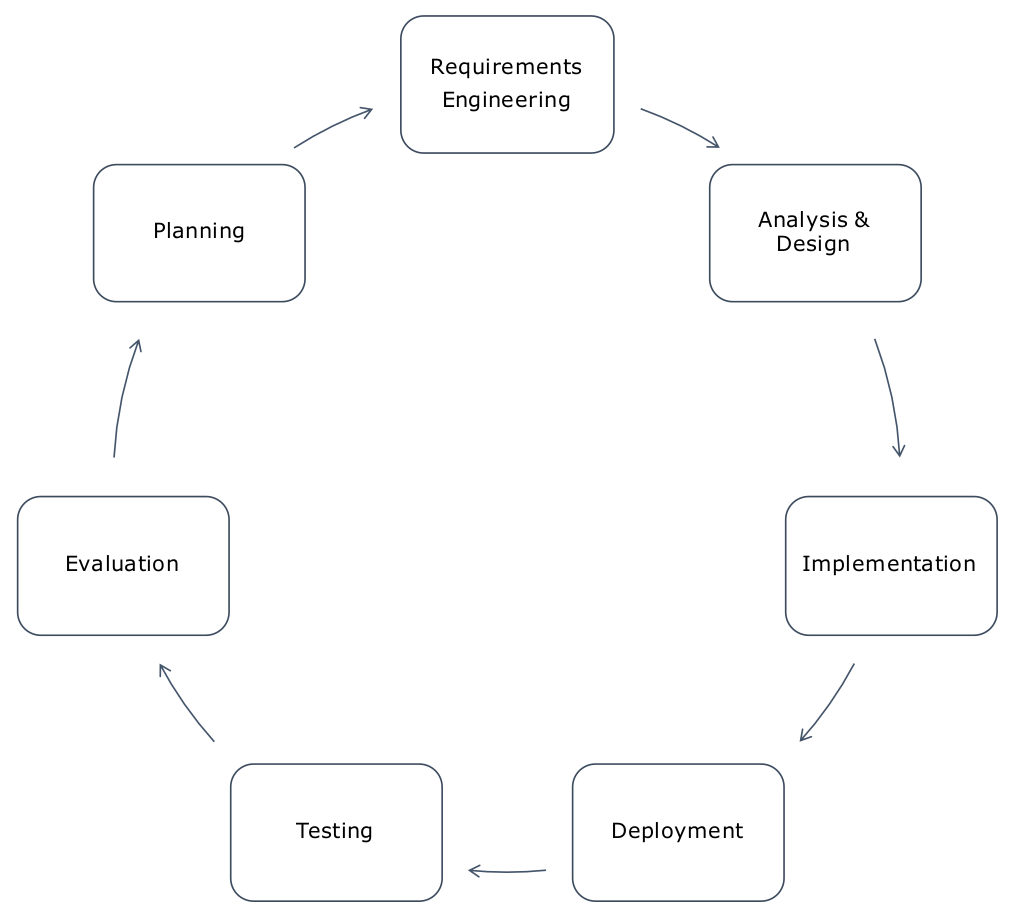
\includegraphics[width=0.8\textwidth]{images/iterative_se_process.png}
\caption{Iterativer Software Engineering Prozess. Aus 
\protect\citeflow{changes_in_requirements_engineering}}
\label{fig:iterative_se_process}
\end{center}
\end{figure}

Aus \citepara{changes_in_requirements_engineering}
\begin{itemize}
	\item Vergleich zwischen zwei Modellen des RE.
	\item Während Updates früher kostenlos (kleinere Updates) oder größere 
Updates (kostenpflichtiger Neuerwerb) waren, mieten Kunden im Cloud Umfeld eine 
Software und erwarten Updates.
	\item Bei einer Migration zu einem Service-Oriented-Architecture 
Modell, werden Teile aus einer Software geschnitten und über eine Schnittstelle 
als Dienstleistung angeboten. Daher wird in der Regel versucht, die meisten 
Funktionalitäten zu übernehmen. Für mehr Informationen: 
\pcite{}{}{service-oriented_migration}
	\item Es gibt drei Nicht-Funktionale Anforderungen die aus SaaS 
entstehen: 
\begin{enumerate}
	\item Software muss in einer Cloud-Umgebung gehostet werden. Dies 
hat Einfluss auf die Themen Sicherheit, Vertraulichkeit, Verschwiegenheit, 
Compliance.
	\item In der Regel eine webbasierte Anwendung, d.h. es werden übliche 
Internetprotokolle verwendet. Dies hat Einfluss auf die Themen: Multi-Tenancy, 
User Concurrency, Konfigurierbarkeit, Skalierbarkeit, Verlässlichkeit, 
Leistungsfähigkeit, Verfügbarkeit, Kompatibilität, Interoperabilität, 
Portabilität, Effizienz, Direktheit
	\item In der Regel ist eine Bedienung über den Browser möglich, die 
Installation einer zusätzlichen Anwendung nicht erforderlich
\end{enumerate}
	\item Business Changes erforderlich. Näheres 
\pcite{}{}{transitioning_to_saas}. Update Mechanismen, Non-disruptive Upgrade 
Modelle
	\item \pcite{}{}{requirements_engineering_process_for_saas_cloud_env} 
Neuer Stakeholder: Cloud Service Provider. Schlagen Checkliste für neue 
Stakeholder vor.
	\item Noch mehr Stakeholder Analysten, Grafik Designer, Kunden, 
Marketing, Sicherheitsexperten 
\pcite{}{}{adapting_the_software_engineering_process}
\end{itemize}

\subsubsection{Transformation des bisherigen Requirements-Engineering}
\citeflow{changes_in_requirements_engineering} schlagen die folgenden Schritte 
vor, um die Anforderungsermittlung an die Cloud anzupassen:
\begin{enumerate}
	\item Paradigma sich schnell ändernder Anforderungen etablieren. Die 
Nähe zur agilen Entwicklung und neuen Methoden der Anforderungsermittlung 
sorgen für eine Volatilität der Anforderungen.
	\item Integrieren der Anforderungsermittlung in einen iterativen, 
inkrementellen Software Engineering Prozess. Nicht typisch für die Cloud, aber 
besonders erforderlich aufgrund der volatilen Anforderungen.
	\item Identifizierung und Priorisierung der Stakeholder mit 
systematischen Methoden
	\item Einbeziehung der Kunden in die Anforderungsermittlung mittels 
Feature Requests und Bug Reports sind essentiell um Vorteil aus der 
Cloud-Migration zu ziehen. Nutzer müssen das Gefühl bekommen, Einfluss auf die 
Entwicklung nehmen zu können.
	\item Implementierung von Feedbackmöglichkeiten. Entweder automatisiert 
über die Auswertung von Daten oder über Formulare. 
	\item Nutzen von Mechanismen für unterbrechungsfreie Updates. Nicht 
Administratoren, sondern Entwickler bestimmen den Updatezeitpunkt.
	\item Entwicklung von Möglichkeiten, Software an kleineren 
Nutzergruppen zu testen.
\end{enumerate}


\subsubsection{Unterschiede im Requirements Engineering}
\begin{table}[ht!]
\centering
\begin{longtable}{|p{0.45\textwidth}|p{0.45\textwidth}|}
\hline
\textbf{On-Premise-Software} & \textbf{Software as a Service} \\
\hline %%%%%%%%%%%%%%%%%%%%%%%%%%%%%%%%%%%%%%%%%%%%%%%%%%%%%%%%%%%%%%%%%
Überschaubare Anzahl von Stakeholdern & Viele verschiedene Stakeholder \\
\hline
Keine oder geringe Einbeziehung des Kunden in die Entwicklung & Starke 
Einbeziehung \\ \hline
Geschäftsbeziehung zum Kunden endet mit einmaliger Zahlung & langfristige 
Geschäftsbeziehung \\ \hline
Nutzungserfahrungen nur über spezielle Erhebungen & Direkte Rückmeldung, ggf. 
motiviert durch Hoffnung auf Fehlerbehebung oder neue Features \\ \hline
Regelmäßige, geplante Fehlerbehebung & Sofortige Fehlerbehebung \\ \hline
Keine neuen Features ohne Versionsupgrade & Andauernde Auslieferung neuer 
Features ohne größere Verzögerung \\ \hline
Updates und Upgrade erfordern Downtime & Nahtloser Updateprozess ohne 
Unterbrechung \\ \hline
Upgrades haben größere Auswirkungen und machen Schulungen erforderlich & 
Kontinuierliche Auslieferung weniger disruptiv \\ \hline
Prognose und Test der Akzeptanz schwierig & Alternativen lassen sich an 
kleineren Nutzergruppen testen \\
\hline %%%%%%%%%%%%%%%%%%%%%%%%%%%%%%%%%%%%%%%%%%%%%%%%%%%%%%%%%%%%%%%%%
\end{longtable}
\caption{Unterschiede im Requirementsengineering. Entnommen aus 
\cite{changes_in_requirements_engineering}}
\label{tab:unterschiede_im_re}
\end{table}

\subsubsection{Kategorien und Anforderungen}
Aus \citeflow{requirements_engineering_process_for_saas_cloud_env}:
\begin{description}
	\item[Anforderungen an die Architektur] Passendes Auslieferungsmodell, 
Sicherheit, Privatsspähre, Hohe Verfügbarkeit und Anpassbarkeit. Verschiedene 
Levels von Service Level Agreements (SLA). Sollte zustandslos (niedrige Kosten, 
hohe Zuverlässigkeit und Performanz) sein. Fehlertolerant, umfassende 
Redundanz und Uptime, Strategien für den Fehlerfall. Wiederbenutzbare 
Komponenten. Integration mit Altsystemen, API Anforderungen. 
	\item[Anforderungen aus dem Operativen/an das Verhalten] Leichte 
Anpassbarkeit und Erweiterbarkeit der Interfaces, Daten- und Businessprozesse, 
User Experience, Designanforderungen, Sicherheit und Privatsspähre, 
Verfügabarkeit, Performanz, Interoperabilität, häufige und nicht unterbrechende 
Upgrades. Kapazitätsplanung, Datenmigration, 
	\item[Anforderungen des Managements] Zentralisierte Berichte, 
Monitoring über Einhaltung der SLAs, Rechnungen, Hosting, User Management, 
Kapazitätsplanung und Zuteilung, Datenmanagement, Speicherung, Verarbeitung
	\item[Anforderungen aus Technik/Implementierung] Recruitment, 
Rollenwechsel, 
\end{description}

Schritte, die laut 
\citeflow{requirements_engineering_process_for_saas_cloud_env} im klassischen 
Requirements Engineering ergänzt werden sollten:
\begin{description}
	\item[Testen der Eignung der Cloud-Architektur mit initialen 
Anforderungen]
	\item[Public oder Private Cloud?]
	\item[Passende Cloud Service Provider identifizieren]
	\item[Kosten der Cloud-Lösung abschätzen] Cloudonomics
	\item[Anforderungen dokumentieren] Wekcge Art von physischer und 
persönlicher Sicherheit bietet die CLoud? Wie würden Anwendungen überwacht, die 
in einer Public Cloud? Wie skalierbar wäre die Cloud?
\end{description}

\cite{changes_in_requirements_engineering}


\subsubsection{Anforderungsermittlung}
\subsubsection{Return on Investment (ROI)}
\subsubsection{Total Cost of Ownership (TCO)}
\begin{comment}
\subsection{Phase IV: Migration}
\subsection{Phase V: Tests und Auslieferung}
\subsection{Phase VI: Überwachung und Wartung}
\subsection{Gesamtbetrachtung}
\subsubsection{Agilität}



\begin{comment}
\label{cha:entwicklung}
Dieses Kapitel dient der Entwicklung eines konzeptuellen Rahmens auf Basis theoretischer Grundlagen, vorausgesetzt sie verfolgen einen positivistischen Ansatz. Hierfür leiten Sie Hypothesen aus verschiedenen sinnvoll kombinierten Quellen her. Hierdurch generieren Sie aus bestehendem Wissen neues Wissen, was eine Eigenleistung und somit ein wichtiger Bestandteil Ihrer Arbeit darstellt.

Sollte Ihre Arbeit nicht positivistisch ausgelegt sein, stellt dieser Abschnitt kein Pflichtkapitel der Arbeit dar. Alternativ beschreiben Sie Anforderungen für ein mögliches Konzept oder verzichten vollständig auf dieses Kapitel.

\textbf{Setzen Sie sich frühzeitig mit Ihrem Betreuer in Verbindung, um Ihre Gliederung abzustimmen und mögliche Missverständnisse zu beseitigen.}

Im Folgenden werden einige allgemeine Hinweise zu den Themen richtiges Zitieren und Literaturrecherche gegeben.


\subsection{Quellen und richtiges Zitieren}
Quellen können in Fußnote oder direkt im Text platziert werden. Alles was nicht Ihr eigenes Gedankengut darstellt, muss mit einer entsprechenden Quelle belegt werden. Hierbei können wörtliche und indirekte Zitate verwendet werden. Wörtliche Zitate sind immer mit der Seitennummer der Quelle anzugeben.

Beispiel für ein direktes Zitat:

%\textit{\glqq The case study is a research strategy which focuses in understanding the dynamics present within single settings\grqq} \pcite{}{543}{eisenhardt1989}.

Beispiel für ein indirektes Zitat:

%Eine explorative Fallstudie dient der Gewinnung von neuen Erkenntnissen und der Bildung von neuen Hypothesen über bestimmte Sachverhalte. Durch den Beitrag zum Theorieaufbau ist der Erkenntnisgewinn höher als bei einer reinen deskriptiven Fallstudie. In explorativen Fallstudien werden Phänomene in noch wenig erforschten Gebieten identifiziert und aus erkannten Zusammenhängen neue Hypothesen gebildet \citepara{eisenhardt1989}.

Alternativ kann die Quelle auch im  laufenden Text angegeben werden:

%Nach \citeflow{eisenhardt1989} wird die Wichtigkeit der Fallauswahl oft unterschätzt. Die Fälle können zwar zufällig ausgewählt werden, dies ist aber weder notwendig noch wünschenswert.

Quellenangaben bestehen aus Autor, Jahr und ggf. Seitenangabe. Bei zwei Autoren sind beide Autoren zu nennen, bei mehreren Autoren nur der erste Autor mit dem Zusatz „et al.“.\newpage


\subsection{Zitieren mit Endnoten}
Im Rahmen der Erstellung von Arbeiten am Fachgebiet ISE ist das Literaturverwaltungsprogramm EndNote zu verwenden. Dieses steht auf der \href{http://www.ulb.tu-darmstadt.de/service/literaturverwaltung_start/endnote_ulb/endnote.de.jsp
}{ULB-Seite} zum Download verfügbar.


\subsubsection{Lateinischer Text mit Zitaten für Erstellung des Literaturverzeichnisses}
\label{cha:source:latintext}
%Lorem ipsum dolor sit amet, consectetur adipiscing elit. Sed vitae lacus eu
%augue semper lobortis vitae aliquet leo. Fusce eleifend sodales commodo
%\citepara{eisenhardt1989}. Mauris arcu metus, bibendum sagittis condimentum
%eget, placerat a enim \citepara{baechle2010}. Quisque sit amet sagittis lectus.
%Curabitur sit amet libero eu felis elementum mollis. Nullam odio diam, mollis
%vitae viverra ut, laoreet ut odio. Praesent facilisis suscipit consequat. Morbi
%feugiat rutrum erat, eu sagittis nibh rhoncus nec \citepara{melao2000}.

%In euismod, arcu ut semper adipiscing, nibh odio ullamcorper arcu, ut scelerisque massa magna nec quam \citepara{benlian2013}. Curabitur bibendum nibh eget augue pellentesque iaculis \citepara{sheffi2005}. Praesent iaculis auctor gravida. Quisque congue, magna ut bibendum semper, enim tortor ultrices lorem, ac feugiat tortor lectus nec nunc \citepara{carnap1974}. Pellentesque habitant morbi tristique senectus et netus et malesuada fames ac turpis egestas. Lorem ipsum dolor sit amet, consectetur adipiscing elit. Fusce dignissim, augue a sodales tristique, neque dui mollis arcu, id interdum augue justo sed lacus \citepara{welchering2013}. Vestibulum ante ipsum primis in faucibus orci luctus et ultrices posuere cubilia Curae; Mauris euismod bibendum nulla, sed accumsan urna tempor sed. Etiam eget diam eros, sed aliquet dolor \citepara{broadbent1996}. Phasellus vitae quam in orci convallis pharetra. Donec sit amet imperdiet nisi \citepara{kayser2013}. Sed vel interdum orci. Praesent vulputate, dolor id varius egestas, enim libero cursus neque, a cursus sapien nulla ut augue. Nullam vitae tortor nisl, vitae cursus enim. Suspendisse eget metus ipsum, sit amet varius sem \citepara{shazly2013}.

\subsection{Literaturrecherche}
Anbei eine kurze Auflistung von möglichen Kanälen zur Literaturrecherche.

\textbf{Zu Verwaltung Ihrer Literatur benutzen Sie bitte das Programm EndNote, dieses wird kostenfrei von der TU zu Verfügung gestellt.}

\url{http://www.ulb.tu-darmstadt.de/angebot/service/literaturverwaltung/endnote.de.jsp}

\subsubsection{Angebot der ULB}
\begin{itemize}
\item Universitätsbibliotheken (\url{http://www.ulb.tu-darmstadt.de/})
\item Rechercheangebot der ULB (\url{http://www.ulb.tu-darmstadt.de/recherche/})
\end{itemize}

\subsubsection{Online-Datenbanken und -Bibliotheken}
\begin{itemize}
\item Elektronische Zeitschriftenbibliothek (EZB) \\
(\url{http://rzblx1.uni-regensburg.de/ezeit/fl.phtml?bibid=TUDA})
\item AIS Electronic Library (AISeL)\\
(\url{http://aisel.aisnet.org/})
\item Zeitschriftendatenbank (ZDB)\\
(\url{http://dispatch.opac.ddb.de/DB=1.1/srt=YOP/})
\item Datenbank-Infosystem (DBIS): Literatur- und Fakten-Datenbank\\
(\url{http://rzblx10.uni-regensburg.de/dbinfo/fachliste.php?bib_id=tud})
\item IEEE Xplore \\
(\url{http://ieeexplore.ieee.org/Xplore/dynhome.jsp?tag=1})
\item EBSCO: internationale wirtschafts-wiss. Zeitschriften\\ (\url{http://search.ebscohost.com})
\item Springer-Online: Bücher/Beiträge des Springer Verlags\\
(\url{http://www.springerlink.com})
\item WiSo Net: deutschsprachige Literatur zu Wirtschafts- und Sozialwissenschaften\\
(\url{www.wiso-net.de})

\end{itemize}

\subsubsection{Sonstiges}
\begin{itemize}
\item \textbf{Google Scholar:} Suchdienst für wissenschaftliche Recherchen (http://scholar.google.de)
\item \textbf{Verlagswebseiten} Recherche und den Zugriff auf Zeitschriften- und Zeitungsartikel und E-Books
\item \textbf{Webseiten von Unternehmen} für die Recherche von Unternehmensdaten und-statistiken sowie Unternehmensdatenbanken
\item \textbf{Webseiten von Bundes- und Landesbehörden sowie der EU}
 Statistisches Bundesamt (http://www.destatis.de)
\\Presse- und Informationsamt der Bundesregierung (http://www.bundesregierung.de)
\item \textbf{Webseiten von Marktforschungsinstituten}
(für Marktanteile und Verbraucheranalysen)
\item \textbf{Webseiten von Verbänden und Kammern}
Institut der deutschen Wirtschaft (http://www.deutsche-wirtschaft.de)
\end{itemize}
\end{comment}
%3
%\section{Forschungsmethoden}
\label{cha:method}
Wie die für diese Arbeit gewonnen Informationen in das Ergebnis einflossen, ist 
in Abbildung~\ref{fig:einfluss_forschungsmethoden} dargestellt. Auf Basis der 
Ergebnisse der systematischen Literaturübersicht wurde das Vorgehensmodell 
entwickelt. Anschließend wurde dieses theoretische Modell auf ein Projekt aus 
der Praxis angewandt, um ein modell-ideales Vorgehen aufzuzeigen. Zum Schluss 
wurde dieses ideale Vorgehen mit Erfahrungen aus der Praxis diskutiert und 
erweitert.

\usetikzlibrary{decorations.text}
\usetikzlibrary{calc}
\usetikzlibrary{fit}
\usetikzlibrary{shapes}
\usetikzlibrary{arrows,positioning} 

%\begin{document}
\begin{figure}[h]
\begin{center}
\scalebox{1}{
\begin{tikzpicture}[
	node distance=1.25cm,
	auto,
	pile/.style={
		very thick,
		->,
		>=stealth',
		shorten <=3pt,
		shorten >=3pt
	},
	knoten/.style={
		text width=5cm,
		text centered
	}
]
\node[knoten] (INFOS)  {\textbf{Informationsgewinnung}};
\node[knoten] (ERG) [right=of INFOS] {\textbf{Ergebnisse in dieser Arbeit}};

\node[knoten] (LIT) [below=of INFOS]
{Literaturrecherche\\(Kapitel~\ref{cha:literaturuebersicht})};

\node[knoten] (INV) [below=of ERG, right=of LIT] {};


\node[knoten] (PROJ) [below=of LIT] {Projekt aus 
der Praxis\\(Kapitel~\ref{cha:replyundifms})};

\node[knoten] (VOR) [right=of PROJ, below=of INV] 
{Vorgehensmodell\\(Kapitel~\ref{cha:entwicklung_vorgehensmodell})};


\node[knoten] (IDEAL) [below=of VOR] 
{Modell-ideales Vorgehen\\(Kapitel~\ref{cha:result})};

\node[knoten] (ERF) [below=of PROJ] {Erfahrungen aus 
der Praxis\\(Kapitel~\ref{cha:praxis})};

\node[knoten] (DISK) [below=of IDEAL] 
{Diskussion\\(Kapitel~\ref{cha:diskussion})};

\node[above left = 0.15cm and 0.65cm of ERG] (o) {};
\node[below left = 0.15cm and 0.65cm of DISK] (u) {};

\draw[loosely dotted] (o) -- (u);

\draw[pile] (LIT) -> (VOR);
\draw[pile] (VOR) -> (IDEAL);
\draw[pile] (PROJ) -> (IDEAL);
\draw[pile] (IDEAL) -> (DISK);
\draw[pile] (ERF) -> (DISK);

\end{tikzpicture}
}
\caption{Einfluss der Forschungsmethoden in die Arbeit}
\label{fig:einfluss_forschungsmethoden}
\end{center}
\end{figure}

Die Abläufe der systematischen Literaturrecherche und der Gespräche und 
Workshops werden in den 
Kapiteln~\ref{cha:literaturuebersicht}~beziehungsweise~\ref{cha:praxis} 
dargestellt; Das Praxisprojekt wurde bereits in Kapitel~\ref{cha:replyundifms} 
vorgestellt, weshalb auf eine erneute Vorstellung an dieser Stelle verzichtet 
wird.
\subsection{Theorie: Systematische Literaturübersicht}
\label{cha:literaturuebersicht}
Die systematische Literaturübersicht wurde wie von \citeflow{kitchenham2004} 
vorgeschlagen durchgeführt: Zunächst wurden für jede Forschungsfrage 
Schlüsselwörterund ihre Synonyme identifiziert und anschließend mit booleschen 
Operatoren verknüpft. Die entstandenen Ausdrücke sind in 
Tabelle~\ref{tab:searchstrings}) zu finden und dienten anschließend der 
Recherche in Literaturdatenbanken in Tabelle~\ref{tab:literaturdatenbanken}.
%
% WICHTIG
% Wenn hier eine Frage angepasst wird, muss sie auch in der Datei 
% forschungsfragen.tex angepasst werden
%
\begin{table}[h]
\centering
\begin{tabular}{|l|p{0.35\textwidth}|p{0.55\textwidth}|}
	\hline
	\textbf{\#} & \textbf{Frage} & \textbf{Rechercheausdruck} \\
	\hline
	1 & In welche Aufgaben lässt sich die Migration 
einer On-Premise-Software zu Salesforce unterteilen? & (tasks OR 
needs OR requirements)\newline AND\newline (migration OR adoption)\newline 
AND\newline salesforce
\\
	\hline
	2 & Welche Methoden unterstützen diesen Migrationsprozess? & (methods OR 
standards OR framework) \newline AND\newline 
('cloud migration' OR 'cloud adaption' OR 'salesforce') \\
	\hline
	3 & Wie unterstützt Salesforce die Migration technisch? & (tools OR 
interfaces OR api)\newline AND\newline (migration OR 
adoption)\newline 
AND\newline salesforce\\
	\hline
	4 & Wie wirkt sich die Migration auf die strategische Marktposition aus? 
& (strategy OR market) \newline 
AND\newline 
('cloud migration' OR 'cloud adaption') \\
	\hline
\end{tabular}
\caption{Forschungsfragen und zugehörige Rechercheausdrücke. Angelehnt 
an \cite{exploring_the_factors}
}
\label{tab:searchstrings}
\end{table}



Ausgeschlossen und in der Tabelle vermerkt wurden Literaturdatenbanken, bei 
denen keine Suche mit geklammerten booleschen Ausdrücken möglich ist. Wurden 
Ergebnisse zu einer Frage gefunden, wurde dies mit einem Haken vermerkt; ist 
das Feld leer, gab es keine Treffer.

Außerdem wurden nur Ergebnisse berücksichtigt, die
\begin{itemize}
	\item den Rechercheausdrücken entsprachen.
	\item in deutscher oder englischer Sprache vorlagen.
	\item vollständig vorlagen
	\item in Abstract oder Fazit einen Zusammenhang zu den Forschungsfragen
aufwiesen
	\item seit einschließlich dem Jahr 2010 erschienen sind.
\end{itemize}
 \begin{table}[bh]
\centering
\begin{tabular}{|p{0.4\textwidth}|p{0.1\textwidth}|p{0.1\textwidth}|p{
0.1\textwidth}|}
\hline
  \hfill & \multicolumn{3}{c|}{\textbf{Forschungsfragen}} \\
  \hline
\textbf{Name und URL} & \textbf{1} & \textbf{2} & \textbf{3} \\
\hline
ACM Digital Library \newline \url{http://dl.acm.org/} & $\surd$ & ? & ? \\
	%Frage 2 \newline
	%\st{Frage 1,3,4}: Keine Volltextergebnisse \\
	\hline
	Science Direct \newline \url{http://www.sciencedirect.com/} & ?& 
?& ?\\
	\hline
	Wiley \newline \url{http://eu.wiley.com/} & \multicolumn{3}{c|}{Keine 
booleschen Ausdrücke möglich} \\
	%\st{Frage 1,2,3,4}: Keine Suche mit booleschen Ausdrücken möglich \\
	\hline
	Elektronische Zeitschriftenbibliothek (EZB)\newline
\url{http://rzblx1.uni-regensburg.de/ezeit/fl.phtml?bibid=TUDA} & 
\multicolumn{3}{c|}{Keine 
booleschen Ausdrücke möglich} \\
	\hline
	Compendex \newline
\url{https://www.elsevier.com/solutions/engineering-village/content/compendex} 
& \multicolumn{3}{c|}{Keine 
booleschen Ausdrücke möglich} \\
	\hline
	AIS Electronic Library (AISeL) \newline \url{http://aisel.aisnet.org/} & 
\multicolumn{3}{c|}{Keine 
booleschen Ausdrücke möglich} \\
	\hline
	Zeitschriftendatenbank (ZDB) \newline 
\url{http://dispatch.opac.ddb.de/DB=1.1/srt=YOP/} & ? & ? & ? \\
	\hline
	IEEE Xplore \newline 
	\url{http://ieeexplore.ieee.org/Xplore/dynhome.jsp?tag=1} & 
	? & ? & ? \\
	\hline
	Springer-Online: Bücher/Beiträge des Springer Verlags \newline
	\url{http://www.springerlink.com} & $\surd$ &  &  \\
	\hline
Rechercheangebot der ULB 
\newline \url{http://www.ulb.tu-darmstadt.de/recherche/} & $\surd$ & 
$\surd$ & $\surd$ \\
\hline
%	WiSo Net: deutschsprachige Literatur zu Wirtschafts- und 
%	Sozialwissenschaften \newline \url{www.wiso-net.de} & ? & ? & ? \\
%	\hline
	%EBSCO: internationale wirtschafts-wiss. Zeitschriften \newline 
	%\url{http://search.ebscohost.com} & ? & ? & ? \\
	%\hline
\end{tabular}

\caption{Literaturdatenbanken und für welche Fragen sie herangezogen wurden. 
Quellen: \cite{exploring_the_factors} und \cite{formatvorlage}}
\label{tab:literaturdatenbanken}
\end{table}
% $\surd$

\begin{comment}
\subsubsection{Sonstiges}
\begin{itemize}
\item \textbf{Google Scholar:} Suchdienst für wissenschaftliche Recherchen 
(http://scholar.google.de)
\item \textbf{Verlagswebseiten} Recherche und den Zugriff auf Zeitschriften- 
und 
Zeitungsartikel und E-Books
\item \textbf{Webseiten von Unternehmen} für die Recherche von 
Unternehmensdaten 
und-statistiken sowie Unternehmensdatenbanken
\item \textbf{Webseiten von Bundes- und Landesbehörden sowie der EU}
 Statistisches Bundesamt (http://www.destatis.de)
\\Presse- und Informationsamt der Bundesregierung 
(http://www.bundesregierung.de)
\item \textbf{Webseiten von Marktforschungsinstituten}
(für Marktanteile und Verbraucheranalysen)
\item \textbf{Webseiten von Verbänden und Kammern}
Institut der deutschen Wirtschaft (http://www.deutsche-wirtschaft.de)
\end{itemize}
\end{comment}

\begin{comment}
In diesem Kapitel erläutern Sie ihre Forschungsmethode unter Verwendung von
entsprechenden Quellen.
Begründen Sie auch, warum Sie sich für diese Forschungsmethode entschieden
haben
und warum sie geeignet ist, die vorliegende Forschungsfrage zu beantworten.
\end{comment}
\subsection{Praxis: Workshops und Einzelgespräche}
Es fanden insgesamt drei, jeweils sechsstündige Workshops statt, an denen die 
Entwickler von iFMS, der Projektleiter von iFMS, drei 
Salesforce-Entwickler sowie der Autor dieser Thesis teilnahmen. Thematisiert 
wurde dabei, wie eine Salesforce-Implementierung von iFMS aussehen und welchen 
Umfang sie haben sollte. Die Workshops blieben dabei unbeeinflusst vom in 
dieser Arbeit entwickelten Vorgehensmodell, um zunächst möglichst unverfälschte 
Erfahrungen aus der Praxis einfließen zu lassen.

Um Rückmeldungen zum Vorgehensmodell selbst zu erhalten wurden danach 
vier Einzelgespräche von jeweils etwa eineinhalb Stunden Dauer geführt. 
Die Gesprächspartner werden im folgenden in Hinblick auf ihre Position und 
ihrer Rolle im bisherigen und künftigen iFMS-Umfeld vorgestellt. Außerdem wird 
kurz ihre Aufnahme in den Kreis der Gesprächspartner begründet.

\newcommand{\person}[3]{\begin{description}
                        	\item[Position:] #1
				\item[Beschreibung:] #2
                        	\item[Begründung der Wahl:] #3
                        \end{description}
}
\begin{itemize}
\item \person{Entwickler}{War als Entwickler bei iFMS tätig und soll auch im 
neuen Team tätig sein}{Kann durch seine 
Kenntnisse Anforderungen und Aufwand der SAP-Anbindung, der CAD-Darstellung 
sowie der Verarbeitung der CAD-Dateien abschätzen.}
\item \person{Senior Consultant}{Teamleiter des bisherigen iFMS-Teams und des 
neuen Teams}{Kann durch seine bisherige Verkaufstätigkeit Kenntnisse über den 
 bisherigen Kundenkreis einbringen.}
\item \person{Manager}{Unbeteiligt am Projekt}{Kann seine jahrelange 
Entwicklungserfahrung mit Salesforce einbringen.}
\item \person{Geschäftsführer}{Nicht direkt ins Projekt eingebunden}{Kann 
erhebliche strategische Erfahrungen im Salesforce-Umfeld einbringen.}
\end{itemize}
Die Gespräche wurden vom Autor nicht gezielt gelenkt; es gab keinen 
Fragenkatalog oder Ähnliches. Ziel war es, den Gesprächspartnern die 
Möglichkeit zu geben, beliebige Aspekte zu ergänzen oder alternative 
Betrachtungsweisen aufzuzeigen.
\label{cha:praxis}%4
%\section{Das Projekt: iFMS@Salesforce}
%\section{Forschungsergebnisse}
\label{cha:result}
\begin{comment}
In Kapitel „Forschungsergebnisse“ stellen Sie die Ergebnisse ihrer Arbeit dar.
An dieser Stelle nehmen Sie noch keine Interpretation oder Erläuterung der 
Ergebnisse vor, sondern beschreiben rein deskriptiv ihre Befunde. Eine 
Auswertung findet im nachfolgenden Kapitel statt.
\end{comment}

Das entwickelte Vorgehensmodell soll nun auf ein Migrationsprojekt aus der 
Praxis angewendet werden. Dazu werden zunächst die Firma sowie die 
Rahmenbedingungen des Projektes vorgestellt. Anschließend wird exemplarisch 
eine Vision für das Projekt entwickelt.

\subsection{Beteiligte Unternehmen und das On-Premise-Produkt}
\usetikzlibrary{decorations.text}
\usetikzlibrary{calc}
\usetikzlibrary{fit}
\usetikzlibrary{shapes}
\usetikzlibrary{arrows,positioning} 
\pgfmathsetmacro{\cubex}{4}
\pgfmathsetmacro{\cubey}{2}

\definecolor{light-gray}{gray}{0.80}

\tikzset{
    %Define standard arrow tip
    >=stealth',
    %Define style for boxes
    punkt/.style={
           rectangle,
           rounded corners,
           draw=black, very thick,
           text width=8em,
           minimum height=2em,
           text centered},
    % Define arrow style
    pil/.style={
           ->,
           very thick,
           shorten <=5pt,
           shorten >=5pt,},
    Line/.style={
	dashed,
	very thick
    }
}




%\begin{document}
\begin{figure}[bh]
\begin{center}
\scalebox{1}{
\begin{tikzpicture}

\newcommand{\yOffset}{-1.9*\cubey}
\newcommand{\yOffsetLineBottom}{\yOffset + 0.35*\cubey}
\newcommand{\yOffsetTop}{-0.9*\cubey}
\newcommand{\imgWidthSmall}{0.17\textwidth}
\newcommand{\xOffsetBottom}{0.23*\textwidth}

\coordinate (RO) at (0,0);
\coordinate (LO) at (-\cubex,0);
\coordinate (RU) at (0,-\cubey);
\coordinate (LU) at (-\cubex,-\cubey);
%\draw (RO) -- (RU) -- (LU) -- (LO) -- (RO);
\node[] (reply) at (0,0) 
{
\includegraphics[width=0.45\textwidth]{images/reply.png} };


\node[] (syskoplan) at (0,\yOffset) 
{
\includegraphics[width=\imgWidthSmall]{images/syskoplan.jpg} };
\draw[Line] (0,\yOffsetTop) -- (0,\yOffsetLineBottom);


\node[] (arlanis) at (-\xOffsetBottom,\yOffset) 
{
\includegraphics[width=\imgWidthSmall]{images/arlanis.jpg} };
\draw[Line] (-\xOffsetBottom,\yOffsetTop) -- 
(-\xOffsetBottom,\yOffsetLineBottom);

\node (others) at (\xOffsetBottom,\yOffset) {\Huge{...}};
\draw[Line] (\xOffsetBottom,\yOffsetTop) -- 
(\xOffsetBottom,\yOffsetLineBottom);

\end{tikzpicture}
}
\caption{Das Reply Unternehmensnetzwerk. Eigene Grafik.}
\label{fig:reply}

\end{center}

\end{figure}



Reply ist ein an der italienischen Börse gehandeltes 
IT-Beratungsunternehmen und betrachtet sich als "`Living network"'\ aus 
hochspezialisierten Tochterunternehmen. Seit der Gründung 1996 konnte Reply 
seinen Umsatz auf über 705 Millionen Euro bei 5.245 Angestellten im Jahr 2015 
steigern. Das Netzwerk wuchs und wächst rasch: 2016 wurden bis November drei 
neue Firmen aquiriert. Zwei Tochtergesellschaften, die schon seit mehreren 
Jahren Teil von Reply sind, 
möchte ich genauer vorstellen, da ihre Unternehmensprofile das 
Migrationsprojekt in besonderem Maße beeinflussen.

Die vormalige syskoplan AG, seit dem Erwerb 2010 \pcite{}{12}{replycompprofile} 
Syskoplan Reply, ist ein Spezialist für SAP-Applikationen und 
-Plattformen \pcite{}{10}{replycompprofile} und entwickelt seit 1999 das 
integrierte Facility Management System (iFMS). iFMS verbindet die in SAP 
hinterlegten Daten mit Gebäudeplänen und versucht Prozesse rund um die 
Verwaltung von Immobilien zu unterstützen. Die gewachsene 
Java-Anwendung mit einer Client-Server-Architektur lässt sich inzwischen nur 
noch schwer um von Kunden gewünschte Funktionen erweitern. Auch die Bedienung 
über 
eine zusätzlich zu installierenden Anwendung wirkt in Zeiten, in denen Nutzer 
es gewohnt sind, auch umfangreiche Software über den Webbrowser zu bedienen, 
anachronstisch. Beide Aspekte schränken die zukünftige
Wettbewerbsfähigkeit der Software ein. 

Die ehemalige Arlanis Software AG wurde 2012 von Reply übernommen und ist 
Spezialist für Lösungen auf Basis des Cloud Anbieters Salesforce. Mit 
Salesforce lassen sich Lösungen häufig ganz ohne eigenen Code auf einer 
SaaS-Basis zusammen klicken. Ist doch Code erforderlich lässt er sich auf der 
PaaS-Plattform (Force.com und Heroku) entwickeln, wobei auf per SaaS angelegte 
Datenmodelle und Daten zugegriffen werden kann, auf die externe Anwendungen per 
Web Service zugreifen können. Mit Salesforce1 steht eine App für mobile Geräte 
zur Verfügung; jede Salesforce-Anwendung lässt sich über diese App bedienen. 

Über das Unternehmensnetzwerk von Reply sollen die Stärken beider 
Tochterunternehmen verbunden werden; mit dem Know-How im Bereich Facility 
Management und SAP soll auf Salesforce eine innovative, wettbewerbsfähige 
Anwendung geschaffen werden: iFMS@Salesforce.

Die On-Premise-Anwendung iFMS dient dem Facility Management. Mit ihr lassen 
sich Gebäude, Etagen und Räume verwalten, mieten und vermieten. Dabei werden in 
SAP hinterlegte Informationen wie Raumgrößen, Nutzungsarten, Adressen und 
Kontaktinformationen mit CAD Plänen verknüpft. Um iFMS zu nutzen, müssen 
Unternehmen einen Server bereitstellen und warten, auf dem der Serverteil der 
Anwendung läuft. Außerdem wird ein Datenbankserver benötigt, auf dem iFMS seine 
Daten speichern kann. Auf dem Rechner eines jeden Nutzers muss ebenfalls eine 
Anwendung installiert werden. Ein Screenshot aus Anwendersicht ist in Abbildung 
~\ref{fig:ifms_liegenschaftsbaum} dargestellt. Sie soll nicht im Detail erklärt 
werden, sondern nur die Art und Komplexität der Anwendung andeuten. 

\begin{figure}[!h]
\begin{center}
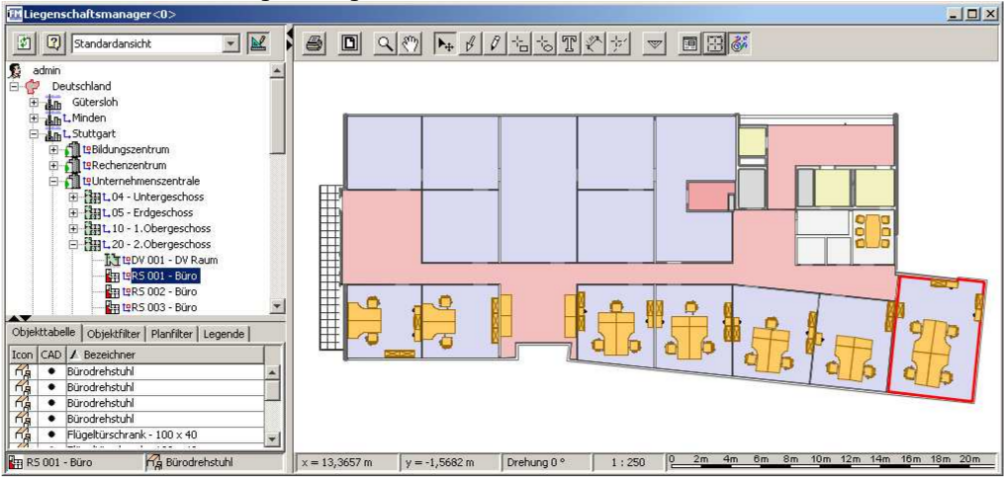
\includegraphics[width=\textwidth]{images/iFMS_liegenschaftsbaum.png}
\caption{Screenshot iFMS aus der 
Benutzerdokumentation (\protect\citeflow{ifms_liegenschaftsmanager}) }
\label{fig:ifms_liegenschaftsbaum}
\end{center}
\end{figure}

Auf der linken Seite lassen sich die Immobilien in einer quasi beliebig 
verzweigten Baumstruktur organisieren. So könnten zu den Kategorien in der 
Abbildung Land, Stadt, Gebäude, Etagen und Räume zum Beispiel noch Kontinente, 
Ländergruppen, Halbetagen oder Raumteile kommen.

Auf der rechten Seite ist der CAD-Plan des Gebäudes bis auf Arbeitsplatzebene 
dargestellt. Arbeitsplätzen können Mitarbeiter, Telefonanschlüsse und beliebige 
Ausrüstungsgegenstände zugeordnet sein. Der Raumplan lässt sich ändern: 
Zwischenwände können gezogen oder entfernt werden. Vertragszugehörigkeiten, 
Raumnutzungsarten und Bodenbeläge lassen sich - auch für jeden Zeitpunkt in der 
Vergangenheit - visualisieren.

\subsection{Vision}
\subsubsection{Realisierung von Chancen}
\begin{description}
	\item[Soziales Element: Vernetzung und Einbeziehung von Nutzern] Die 
Vernetzung zwischen den Nutzern einer Firma erfolgt über Chatter, dem 
Salesforce Äquivalent von Facebook. Der ISV bietet Kundensupport über die 
Salesforce Service Cloud. Entwickler sind für Kunden direkter erreichbar. Durch 
die dort gesammelten Erfahrung können zukünftige Entwicklungsarbeiten 
zielgerichteter erfolgen.
	\item[Analysemöglichkeiten] Der ISV hat Zugriff auf die 
Salesforceinstanzen seiner Kunden. Dadurch kann er Fehlkonfigurationen 
und Fehlbedienungen erkennen, Supportangebote verbessern oder 
Benutzeroberflächen intuitiver gestalten.
	\item[Mobile Nutzung] Mit der Mobile App Salesforce1 ist die Salesforce 
Anwendung auch auf Mobilgeräten nutzbar. Damit ein echter Mehrwert entsteht, 
sollen sich
\begin{itemize}
	\item Rauminformationen wie Belegungen und Ansprechpartner abrufen 
lassen.
	\item Räume buchen lassen.
	\item Schadensmeldungen eingeben lassen und nach Freigabe durch einen 
verantwortlichen Mitarbeiter in einem Auftrag an einen Dienstleister 
resultieren.
	\item über Anwesenheitserkennung Raumtemperatur und Licht regeln lassen.
	\item Räume über ein Indoornavigationssystem finden lassen.
	\item Reiningungspläne einsehen und ändern sowie Sonderreinigungen 
anfordern lassen.
\end{itemize}

	\item[Reduzierte Markteintrittskosten \& Skalierte Märkte] Um die 
Hürden für potentielle Kunden gering zu halten und das Produkt auf diese Weise 
auch für kleine und mittlere Unternehmen attraktiv zu machen, ist die 
SAP-Anbindung optional. Durch die Nutzung des Salesforce Marktplatzes für Apps 
können Kunden das Produkt leicht beziehen und testen.
	\item[Skalierung der Leistung] CAD-Pläne werden nicht mehr lokal 
sondern in der Cloud konvertiert.
	\item[Time to market \& kürzere Releasezyklen] Ein vermarktbares 
Minimum mit einem Bruchteil der Funktionalitäten der komplexen Altsoftware soll 
rasch entwickelt und vermarktet werden. Indem weitere Entwicklung auf den 
Markterfahrungen beruht, wird schnell viel Wert für Kunden geschaffen.
	\item[Alternativen am Kunden testen] 
	\item[Wartung einer einzigen Version] Es gibt einen einzigen 
Softwarestand auf Salesforce der in besonderem Service für Kunden angepasst 
wird. 
	\item[Standardisierte Komponenten] Standardisierte Komponenten lassen 
sich auf dem Salesforce App Marktplatz beziehen. Beispiel dafür ist die 
nahtlose Anbindung an Amazons Dateispeicher S3. Zu prüfen ist auch, ob sich 
Import, Anzeige, Veränderung, Export von CAD Dateien über eine eingekaufte 
Komponente realisieren lassen, da das Unternehmen in diesem Bereich keine 
Kernkompetenz besitzt.
	\item[Stetige Umsätze] Durch ein Preismodell in dem pro Nutzer und 
Monat abgerechnet wird, lassen sich stetige Umsätze generieren.
	\item[Verkauf an Fachabteilungen] Im Marketing soll ein Schwerpunkt 
darauf gelegt werden, Fachabteilungen direkt zu erreichen, zum Beispiel bei 
Fachtagungen einschlägiger Themen. Idealerweise lassen sich kleine Firmen 
erreichen, die das Thema Liegenschaftsmanagement bisher ohne 
Softwareunterstützung bewältigt haben. Sind Fachabteilungen überzeugt lässt 
sich das Produkt ohne Eingriffe in die IT-Landschaft vor Ort nutzen.
\end{description}

\subsubsection{Vermeidung von Risiken}
\begin{description}
	\item[Hohe Kosten durch Pay-per-Use] Da das Produkt wie Salesforce auch 
pro Nutzer und Monat abgerechnet werden soll, sind Kosten absehbar.
	\item[Lock-in Effekte]
	\item[Komplexität unbedacht gekoppelter Komponenten]
	\item[Datenmigration]
	\item[Leistungstransparenz]
	\item[Geringere Umsätze]
	\item[Geringere Anpassbarkeit]
	\item[Organisatorische und strukturelle Umbrüche]
	\item[Updatefrequenz und Agilität]
\end{description}
%5
%\section{Diskussion des modellierten Vorgehens aus praktischer Sicht}
\label{cha:diskussion}
\begin{comment}
Im vorletzten Abschnitt diskutieren Sie Ihre Ergebnisse und stellen den Beitrag 
für die Praxis und für die Forschung dar. Gehen Sie auch auf die Einschränkungen 
Ihrer Arbeit ein.
\end{comment}
Im folgenden werden die in den durchgeführten Einzelgesprächen identifizierten 
Unterschiede zwischen dem tatsächlichen und dem aus dem Modell heraus 
vorgeschlagenen Vorgehen vorgestellt und aufgezeigt, an welchen Stellen und in 
welche Richtungen das Modell erweitert werden müsste.

\subsection{Vermarktung als Projekt}
Der wesentlichste Unterschied zwischen dem vorgeschlagenen und 
tatsächlichen Vorgehen besteht in der Vermarktung. Das mit dem Modell 
erarbeitete Vorgehen sieht vor, Kunden dauerhaft zu binden und dauerhafte 
Umsätze zu generieren. Diese dauerhafte Bindung will Arlanis Reply aus 
strategischen Gründen mittelfristig abbauen, da mit ihr ebenso dauerhafte 
Verpflichtungen eingehen: Kunden erwarten sich von ihren regelmäßigen Zahlungen 
auch stetige Verbesserungen, die aus Sicht des Managements einen 
unverhältnismäßig hohen Aufwand bedeuten. Deshalb will Arlanis iFMS@Salesforce 
in Form einzelner Projekte verkaufen. Anstatt eine fertige Basisversion und 
gegebenenfalls CAD-/SAP-Erweiterungen im Salesforce Marktplatz zu kaufen, 
erhält der Kunde gegen eine einmalige Zahlung eine Software, die von 
Arlanis-Consultants und -Entwicklern in dessen Salesforceumgebung eingerichtet 
wird. 
Jede Erweiterung und Verbesserung muss vom Kunden beauftragt und bezahlt werden.
\begin{table}[h]
\centering
\begin{tabular}{|p{0.47\textwidth}|p{0.47\textwidth}|}
\hline
\textbf{Vorgeschlagenes Vorgehen:} & \textbf{Tatsächliches Vorgehen} \\
\hline
Vermarktung eines weitgehend standardisierten Produktes & Vermarktung eines für 
den Kunden angepassten Produktes \\
\hline
Bezug über Salesforce-Marktplatz & Produkt wird für den Kunden in 
seiner Installation eingerichtet \\
\hline
Drei Komponenten: Basis, CAD und SAP & Monolithische Architektur, die den 
Wünschen des Kunden entspricht \\
\hline
Kunden erhalten über Marktplatz immer die aktuellste Version & Kunden erhalten 
nur Anpassungen und Updates für iFMS@Salesforce, wenn sie dafür zahlen (von Updates
an der Salesforce-Plattform abgesehen) \\
\hline
Entwicklung, ohne konkreten Kunden für das Produkt zu haben & Entwicklung 
eines jeden Features ausschließlich, wenn es zahlenden Kunden gibt, der 
Entwicklung in Auftrag gibt \\
\hline
\end{tabular}
\caption{Unterschiede zwischen tatsächlichem und vorgeschlagenem Vorgehen}
\label{tab:unterschiede_im_vorgehen}
\end{table}
Aufgrund des im Vergleich zum modellierten Vorgehen geänderten 
Geschäftsmodells, ändert sich das gesamte Produkt (Vgl. 
Tabelle~\ref{tab:unterschiede_im_vorgehen}): Es muss keine allgemein 
funktionierende Basisversion geschaffen werden, die Kunden dazu animiert, 
Erweiterungen zu kaufen, da eine monolithische, auf die jeweiligen 
Kundenbedürfnisse abgestimmte Architektur gewählt wird.

Im Sinne dieser Ausrichtung begann die tatsächliche Entwicklung nicht in der 
Hoffnung das Produkt einmal vermarkten zu können, sondern mit einem konkreten 
Kunden (K), der bereit war für die Entwicklung einer auf ihn angepassten 
Version von iFMS@Salesforce zu zahlen. Bei der künftigen Entwicklung 
beziehungsweise Anpassung von iFMS@Salesforce für andere Kunden soll auf diese 
für K entwickelte Basis zurückgegriffen werden. Für andere Kunden getätigte 
Entwicklungen fließen aber nicht automatisch zurück an K, sondern werden diesem 
in einem Angebot zum Kauf vorgeschlagen.

Aus dieser Einzelvermarktung folgt, dass die gesammelten Ideen dem Kunden zwar 
vorgeschlagen werden können, die Implementierung aber von dessen 
Zahlungsbereitschaft abhängt.

Diese Erfahrung bestätigt das enge Wechselspiel zwischen dem Geschäftsmodell, 
dem geplanten Leistungsumfang sowie der Chancen und Risiken.

\subsection{Skaleneffekte}
Während der Modellvorschlag auf die Erzielung von Skalenerträgen durch die 
Vermarktung auf dem Salesforce Marktplatz setzt, sind aufgrund der Vermarktung 
als Projekt Verkauf, Anpassung und Training der Endnutzer weiterhin sehr 
personalintensiv, die Skalierbarkeit des Geschäftsmodells dadurch 
eingeschränkt. 

Durch die Vermarktung als Projekt steigt für den Kunden die Investition und mit 
ihr das Risiko. In Folge werden -- anstatt das Produkt direkt an die 
Fachabteilungen zu vermarkten -- weiterhin in vielen Gremien langwierige 
Verhandlungen um den Leistungsumfang geführt, die in Lasten- und Pflichtenheften 
resultieren. Mit diesem Verlust an Agilität geht auch ein weiterer Verlust an 
Skalierbarkeit einher. Anstatt einem Kunden schnell die Lösung zu liefern und 
Umsätze zu generieren, muss der ISV erheblich in die Verhandlungen investieren, 
ohne das der Vertragsabschluss gesichert wäre.

Während eine personalintensive Wertschöpfung charakteristisch für 
Beratungsunternehmen ist, könnte Arlanis überdenken, ob der direkte Verkauf an 
Fachabteilungen durch Minderung des Risikos für den Kunden durch die 
Realisierung von Cloud-Vorteilen forciert werden könnte. 

\subsection{Anforderungsermittlung und -umfang}
Im Zuge der Anforderungsermittlung für iFMS@Salesforce traten 
unterschiedlichen Ansichten zwischen den Entwicklern (des alten iFMS) und 
dem Management zu Tage. Während den Entwicklern eine möglichst elegante 
Architektur am Herzen lag, die es in Zukunft ermöglichen würde, die gleiche 
Basis für eine Vielzahl von Kunden nutzen zu können, war dem Management vor 
allem eine schnelle und den Kunden K zufriedenstellende Lösung (Minimum viable 
product) wichtig. Eine allgemeine Lösung würde -- da K dafür nicht zahlt -- 
zunächst auf Kosten für Arlanis Reply hinauslaufen. Man war nicht bereit für 
eventuelle zukünftige Kunden in Vorleistung zu treten. Eine Entscheidung die vom 
Modell dieser Arbeit gestützt wird, um das Risiko für den ISV zu minimieren.

Ein ähnlich gelagertes Problem entstand aus der sentimentalen Bindung der 
Entwickler zu ihrer bisherigen Arbeit. Mit dem Übergang zu Salesforce wird der 
größte Teil ihrer bisherigen Arbeit nicht mehr benötigt. Aufgrund des im 
Vergleich zum alten iFMS reduzierten Leistungsumfangs wird zudem die neue 
Software viel weniger Fähigkeiten haben. Es zu erreichen, dass die Entwickler 
trotzdem überzeugt hinter dem neuen Produkt stehen, stellt eine Herausforderung 
dar, die in dem hier vorgestellten Modell nicht berücksichtigt wird.

\subsection{Forschungsbeitrag}
Diese Arbeit konnte mit Ihren Ergebnissen zeigen
\begin{enumerate}
	\item welche Merkmale, Chancen und Risiken bei der Migration in die 
Cloud zu berücksichtigen sind,
	\item wie diese Merkmale die strategische Ausrichtung und das 
Geschäftsmodell von Softwareherstellern beeinflussen und
	\item wie diese Merkmale den Migrationsprozess von Softwareherstellern 
beeinflusst
\end{enumerate}
und damit die in Kapitel~\ref{cha:einleitung} gestellten Forschungsfragen 
beantworten, sowie wechselseitige Einflüsse zwischen Geschäftsmodell, Strategie 
und Merkmalen aufzeigen.

Der Katalog der Cloud-Merkmale half bei einem Projekt aus der Praxis als 
Checkliste zu bedenkender Aspekte dabei, das geplante Vorgehen systematisch zu 
überprüfen. Dass die Ergebnisse zwischen vorgeschlagenem und tatsächlichen 
Vorgehen deutlich voneinander abweichen, ist unerheblich. Ziel dieser Arbeit war 
es, ein Vorgehensmodell zu entwickeln, das die Migration in die Cloud 
unterstützt. Dies geschieht indem Fragen aufgeworfen und Herausforderungen 
aufgezeigt werden, die Unternehmen für ihre Projekte individuell beantworten 
müssen. 

Auch wenn in dieser Arbeit Salesforce.com als Cloud-Anbieter aufgrund des 
Projektes aus der Praxis im Vordergrund stand, beschränkt sich das Projekt 
keineswegs auf diesen Anbieter. Tatsächlich sind einige Chancen der Cloud bei 
Salesforce technisch ausgeschlossen oder eingeschränkt. Zum Beispiel lassen 
sich bei Salesforce nicht automatisch verschiedene Implementierungsalternativen 
an Kunden testen und auswerten. 
Womöglich lässt sich auch die Entscheidung für 
einen Cloud-Anbieter fundierter treffen, indem verglichen wird, wie gut die 
einzelnen Anbieter die Realisierung der Chancen und die Vermeidung der Risiken 
unterstützen. Dies bleibt jedoch in einer anderen Arbeit zu prüfen.

%6
%%\addtocontents{toc}{\protect\newpage}
\section{Zusammenfassung und Ausblick}
\label{cha:fazit}
% Wohin sind wir gekommen
Mittels einer Literaturanalyse konnte ein theoretisches Vorgehensmodell 
entwickelt werden, das ISV bei der Migration bestehender On-Premise-Anwendungen 
in die Cloud unterstützt, indem es Merkmale, Chancen und Risiken der Cloud 
identifiziert sowie ihre Wechselseitigen Einflüsse zu Geschäftsmodell und 
Strategie aufzeigt. 

Das entwickelte Vorgehensmodell wurde auf ein Projekt aus der Praxis 
angewendet, indem eine Cloud-Vision des bestehenden On-Premise-Produktes 
geschaffen wurde, die versucht Vorteile der Cloud weitestgehend zu realisieren 
und Risiken zu meiden. Um bei der Erstellung der Vision nicht den im 
Unternehmen gewohnten Pfaden zu folgen, wurde an dieser Stelle zunächst 
bewusst darauf verzichtet, Meinungen und Erfahrungen einzuholen.

Dies geschah bei der abschließenden Evaluation des Modells, bei der die Vision 
der Umsetzung mit dem tatsächlichen Vorgehen verglichen wurde. Dabei zeigte 
sich, dass das Modell geeignet ist, um eine Migration systematisch zu planen 
oder eine bestehende Planung zu analysieren. Objekt der Planung beziehungsweise 
der Analyse ist dabei nicht nur der Leistungsumfang der zu gestaltenden 
Cloud-Software sondern in mindestens ebenso großem Maße das Geschäftsmodell und 
die Unternehmensstrategie. Es wurde gezeigt, wie bedeutend die 
Wechselseitigen Einflüsse (Vgl. Abbildung~\ref{fig:wechselseitige_einfluesse}) 
sind, dass der Leistungsumfang an der unternehmerischen Strategie auszurichten 
ist und die Möglichkeiten der unternehmerischen Strategie von realisierbaren 
Merkmalen abhängen.
%\documentclass[border=10pt]{standalone}

\usetikzlibrary{decorations.text}
\usetikzlibrary{calc}
\usetikzlibrary{fit}
\usetikzlibrary{shapes}
\usetikzlibrary{arrows,positioning} 
\pgfmathsetmacro{\cubex}{4}
\pgfmathsetmacro{\cubey}{2}

\definecolor{light-gray}{gray}{0.80}

\tikzset{
    %Define standard arrow tip
    >=stealth',
    %Define style for boxes
    punkt/.style={
           rectangle,
           rounded corners,
           draw=black, very thick,
           text width=8em,
           minimum height=2em,
           
           text centered},
    % Define arrow style
    pil/.style={
           ->,
           very thick,
           %shorten <=2pt,
           shorten >=2pt,},
    sepLine/.style={
	dashed,
	very thick
    }
}


\tikzstyle{b} = [rectangle, draw, node distance=5cm, text 
width=9em, text centered, rounded corners, minimum height=4em, thick]
\tikzstyle{c} = [rectangle, draw, minimum height=15em, minimum width=10em, 
dashed]
\tikzstyle{l} = [draw,thick]

%\begin{document}
\begin{figure}[bh]
\begin{center}
\scalebox{1.0}{
\begin{tikzpicture}[auto]
    \node[b] (S) {Strategie};
    \node[b,below left of=ISV] (G) {Geschäftsmodell};
    \node[b,below right of=ISV] (M) {Cloud-Merkmale, -Chancen und -Risiken};
    
    
   \draw (S)
   edge[pil,<->] (G)
   edge[pil,<->] (M);
   
   \draw (M) edge[pil,<->] (G);
    
 
\end{tikzpicture}
}
\caption{Wechselseitige Einflüsse zwischen Strategie, Geschäftsmodell und 
Cloud-Merkmalen}
\label{fig:wechselseitige_einfluesse}
\end{center}
\end{figure}
Es erscheint vernünftig anzunehmen, dass Migrationsprojekte bei denen 
systematisch Chancen und Risiken der Cloud bedacht wurden wirtschaftlich 
erfolgreicher sind als jene, bei denen dies nicht geschah. Die empirische 
Überprüfung dieser Annahme bleibt jedoch zu erbringen. Ebenfalls 
überprüfenswert scheint die Vermutung, dass sich die Liste der Cloud-Merkmale 
dazu eignen könnte, passende Cloud-Anbieter zu identifizieren. Dies könnte 
geschehen, indem die Cloud-Anbieter darin vergleichen werden, wie gut sie den 
ISV oder ihre Kunden im Allgemeinen darin unterstützen, die identifizierten 
Chancen zu realisieren und die Risiken zu meiden.

Thematisch lediglich am Rande gestreift wurden soziale und organisatorische 
Aspekte. Auch wenn Menschen, die beruflich einer Tätigkeit aus der IT nachgehen 
Kurzlebigkeit gewohnt sind, steigert sich die Geschwindigkeit des Wandels auf 
dem Weg in die Cloud erheblich. Es ist eine Frage an Projektleiter, wie die 
bereits hohe Geschwindigkeit und Agilität weiter gesteigert werden kann, um im 
Cloud Zeitalter weiter wettbewerbsfähig zu bleiben. Ebenfalls wirtschaftlich 
spannend ist die soziale Nachhaltigkeit: Wie lassen sich stabile Teams bilden, 
die die gestiegenen Anforderungen bewältigen können? Wie lassen sich dabei 
Überforderungen und Burnouts vermeiden? Gerade zu Teams historisch gewachsener, 
größerer Projekte dürften -- wie im Beispielprojekt dieser Arbeit -- 
Mitarbeiter gehören, die bisher wenig oder gar keine Erfahrungen mit der 
Cloud besitzen und sich nun im Wettbewerb mit einer sehr viel höheren 
Innovationsgeschwindigkeit sehen. Um weder diese Mitarbeiter noch ihr Know-How 
bei der Migration zu verlieren, müssen Gegenmaßnahmen getroffen 
werden. Wie diese Maßnahmen aussehen, muss in einer anderen Arbeit beantwortet 
werden.

Wenn Kritiker die Cloud als "`alten Wein in neuen Schläuchen"' 
\pcite{}{231}{softwareindustrie2015} beschreiben unterliegen sie einem 
gewaltigen Trugschluss: Die Cloud erhöht die Erwartungen, die Endanwender 
an Software haben in Hinblick auf Preis, Geschwindigkeit, Einfachheit, 
Flexibilität und Effizienz. Ihre ständige Verfügbarkeit wird die Gesellschaft 
immer weiter durchdringen. Softwarehersteller stehen vor der Herausforderung, 
den Wandel nicht nur in technischer, bilanzieller und strategischer Hinsicht zu 
meistern: Auch die Organisation und Kultur des Unternehmens muss überdacht 
werden.
\begin{comment}
Zuletzt fassen Sie Ihre Arbeit kurz zusammen und stellen Ihre wichtigsten 
Schritte, Ergebnisse und Befunde dar. Geben Sie auch einen Ausblick auf mögliche 
anknüpfende Forschungsarbeiten. Außerdem findet sich hier Platz für eine 
kritische Hinterfragung einzelner Teilaspekte und auch für Ihre eigene Meinung.

\subsection{Offene Forschungsfragen}
\begin{itemize}
	\item Wie kann sich ein ISV und ein Softwarebetratungsunternehmen auf 
die strukturellen Änderungen durch die 
Cloud-Migration bei seinen Kunden einstellen?
	\item Die identifizierten Chancen und Risiken hatten Auswirkungen im 
Bereich Visionsentwicklung/Strategie und der Anforderungsermittlung. Wie sind 
die anderen Phasen betroffen.
	\item Einflüsse der Cloud auf Marketing, Strategie und Geschäftsmodell
\end{itemize}

\subsection{Schwierigkeiten}
Trennung zwischen Kundensicht und ISV-Sicht. Siehe Dreieck.




\subsection{Abgabedokument}
% Was wurde in der Arbeit alles gemacht
% Roten Faden aufgreifen
% TODO Pr�sens oder Pr�teritum
\textbf{Abschlussarbeiten} (Bachelor-, Master-, Diplomarbeit) sind in zweifacher 
Ausführung, einseitig bedruckt und gebunden abzugeben. Dazu auf CD die 
Abschlussarbeit in digitaler Form (z.B. Word und PDF), inkl. der 
Endnote-Projektdatei und der Grafiken. 
\end{comment}
\pagenumbering{Roman}
\bibliography{bibliography/referenzen}
%%
%
%
%Appendix
%
%

\appendix

\section{Anhang}
\label{app:crawldata}
Anhang falls notwendig.
%\section{Ideen}
\subsection{Einleitung}
Benlian SaaS 2010: Chancen und Risiken für diesen Anwendungsfall aus Anwendersicht prüfen. In Softwareindustrie werden die einzelnen Chancen und Risiken genauer ausgeführt. ~S. 236
Auch Chancen und Risiken aus Anbietersicht. Softwareindustrie: S: 240 => Verweis auf Benlian 2010, S. 233 \\
Wind: Eval. und Auswahl von Enterprise Cloud Services: Konkretisierung von Zieldimensionen (Flexibilität, Kosten, Leistungsumfang  \& Leistungsfähigkeit, Service \& Cloud Management, IT-Sicherheit \&
Compliance, Ausfallsicherheit \& Vertrauenswürdigkeit). Ab Seite 103. Anforderungsrahmen für die Zieldimensionen und den einzelnen XaaS-Arten. Ab S. 122. Viele Definitionen für Cloud.

Benlian Opportunities and risks of saas 2011: Sicherheit ein Hauptfaktor bei Entscheidung für oder gegen SaaS. Taxonomy of it security risks als Checkliste zur Identifikation von Risiken in bestimmtren
Szenarien. \\

Softwareindustrie: Simple Definition für Cloud aus Standard. \\

Ackermann, Tobias: IT Security Risk Management. Kapitel 5 enthält Empfehlungen für Risk Identification, - Quantification, - Treatment, - Review and Evaluation, - Cloud Computing Providers. S. 22-23 enthält
Beschreibung der Risiken im Cloud Kontext. \\

Key players in the cloud computing industry 
\pcite{}{4}{cloud-computing_the_business_perspective}\\



\subsection{Gamechanger Cloud}
"`What is it about cloud that makes it a game-changer? It
is reported that the business at large find cloud’s affordable,
flexible, on-demand, elastic delivery method, to be extremely
beneficial"'
-- \pcite{}{}{cloud_based_next_generation_service_and_key_challenges}


\subsubsection{Lifecycle}
Aus \citeflow{cloud_based_next_generation_service_and_key_challenges}
\begin{description}
	\item[Design] RE und Design des Dienstes.
	\begin{description}
	\item[Interoperabilität] Unter anderem Amazon, Google, Microsoft,
VMWare und Salesforce bieten Cloud-Plattformen zur Anwendungsentwicklung an.
Bei Nutzung einer solchen Plattform kann nachhaltige Interoperabilität, gerade
bei Nutzung einer privaten oder hybriden Cloud ein Faktor sein.
	\item[Information Centric Design] Bei der Nutzung durch Kunden
anfallende Informationen sollten ständig ausgewertet werden und möglichst in
Echtzeit in zukünftige Entscheidungen einfließen.
\end{description}
	\item[Engineering] Entwicklung, Testen und Operationalisierung \\
	\item[Deployment]
	\item[Usage Measurement]
	\item[Support und Wartung] Informationen, die im Support gesammelt
werden, werden zur Weiterentwicklung genutzt.
	\item[Experience] Um Kunden zu halten, muss die User Experience
verbessert werden
\end{description}

\subsubsection{Towards Modelling a Cloud Applications Life Cycle}
Aus \citeflow{towards_modelling_a_cloud_applications_life_cycle}
\begin{itemize}
	\item Bisherige Life Cycle Modelle fokussieren die Sicht der IT. Es fehlt
	ihnen an einer angemessenen Betrachtung wirtschaftlicher Aspekte.
	\item Schritte im Life-Cycle:
	\begin{itemize}
		\item Business Case Definition
		\item Decision Phase
		\item Design Phase
		\item Test-driven Development Phase
		\item Deployment
		\item Operations (monitoring, updates, resource adaptions, Decommissioning)
	\end{itemize}
	\item Gründe in die Cloud zu gehen:
	\begin{itemize}
		\item Finanzielle Vorteile
		\item Wettbewerbsvorteile
		\item Flexibilität durch On-Demand und self-service
		\item Geringere Risiken
	\end{itemize}
	\item Identifizierte Risiken
	\begin{itemize}
		\item Sicherheit und Haftungsfragen
		\item Technische Probleme
		\item Fehlende Standards
	\end{itemize}
	\item Literatur zu Cloud und Marketing konzentriert sich auf technische
	und finanzielle Faktoren im Deployment und vernachlässigt die Supply Chain
	des Unternehmens und die Auswirkungen auf das Unternehmen selbst
	\item Die Cloud ermöglicht es einem Unternehmen unabhängig von seiner Größe,
	spezialisierte, hochwertige IT-Dienstleistungen in Anspruch zu nehmen.
	\item Die Cloud ist eine ``disruptive innovation'', ein ``new Market'', auf dem IT als Dienstleistung eingekauft wird. Dieser Markt erfordert einen grundlegenden, kulturellen Wandel, mit dem die IT gesehen wird.
	\item Opportunities and Impact
	\begin{itemize}
		\item Verpasste Gelegenheiten durch Über- oder Unterprovisionierung vermeiden
		\item An variable Nachfrage angepasste Dienstleistung
		\item Das Verfolgen von wachsenden oder völlig neuen Märkten
		\item Tätigkeiten schneller und günstiger durchführen
		\item Entkoppeln des Kerngeschäfts von unterstützenden Dienstleistungen
		\item Höhere Umsätze durch amortisierende Skaleneffekte
		\item Höhere Umsätze durch höhere Reichweite
	\end{itemize}
	\item Unternehmen, die in die Cloud gehen, müssen sich den Auswirkungen auf Strategie, Business Model und Unternehmensstruktur bewusst sein.
\end{itemize}


\subsubsection{Service Migration -- Herausforderungen}
Aus \citeflow{cloud_based_next_generation_service_and_key_challenges}
\begin{itemize}
	\item Was für Auswirkungen hat das neue pay-per-use-Modell?
	\item
\end{itemize}

\subsection{Charakteristika Enterprise Applications}
Aus \citeflow{cloudward_bound_planning_for_beneficial_migration}:\\
Bestehen in der Regel aus mehreren Layern (MVC -- Datenbanken, Frontend,
Logik), sind in der Regel aber viel komplexer als dieses dreischichtige Modell,
da jede Schicht aus mehreren, miteinander interagierenden Komponenten aufgebaut
sein kann. \\
Unternehmensanwendungen könnten von zwei verschiedenen Nutzergruppen nutzbar
sein: Unternehmensinterne und -externe Personengruppen.

\subsection{Assessment und Guidelines}
Aus \citeflow{challenges_and_assessment_in_migrating}: \\
\subsubsection{Assessment}
\begin{description}
	\item[Gründe für die Migration] Es ist wichtig die Gründe für die
Migration sowie Anforderungen und Rahmenbedingungen zu kennen, um ihnen zu
genügen.
	\item[Analyse der Anwendungsumgebung] Alle Programme, Skripte und
Interfaces listen, die auf die Anwendung zugreifen.
	\item[Analyse der neuen Umgebung] Welche Ressourcen werden benötigt?
	\item[Design und Analyse der Architektur] Analyse der Architektur der
bestehenden Anwendung mit allen Bibliotheken, Programmen und Plattformen
	\item[Migrationstools] Kleine Proof-of-Concept-Projekte um
Migrationstoosl nach Effizienz, Genauigkeit und Optionen testen.
\end{description}
\subsubsection{Guidelines}
\begin{description}
	\item[Interoperabilität und Zusammenstellen] Nutzen von Schnittstellen
wie der RESTful API.
	\item[Vermeiden des Lock-in Effektes]
	\item[Modellierung des Dienstes und Cloud Deployment Artefakte] Cloud
Modellierungsnotationen sind nützlich.
	\item[Legacy Software verpacken] Es ist unter Umständen einfacher,
praktikabler, sicherer und flexibler Legacy Anwendungen virtualisiert in die
CLoud zu migrieren und über eine Schnittstelle verfügbar zu machen.
	\item[Ausbalancieren von Kosten und Reifegrad] Die Risiken junger,
eventuell unreifer Software sollten in den Aspekt Kosten einbezogen werden.
\end{description}



\subsection{Migrating to -- or away from the public cloud}
Aus \citeflow{migrating_to_or_away_from_the_public_cloud}:
\begin{itemize}
	\item Bei ``Cloud migration'' zwischen Migration der Architektur oder der Operationen.
	\item Migration der Architektur: Migrieren der bestehenden Anwendung zu einer skalierbaren, cloud-bereiten Architektur, häufig unter der Verwendung neuer Programmiersprachen wie Googles Go oder Apples Swift und/oder neuen Komponenten wie NoSQL-Datenbanken.
	\item Migration der Operationen: Verschieden einer cloud-ready Anwendung von der Private in die Public Cloud oder umgekehrt.
	\item Umdenken erforderlich: Bestehende Anwendungen besitzen häufig eine monolithische Natur, bei der das Neuschreiben einer Zeile Code die gesamte Anwendung beeinträchtigen kann. Deshalb sind nach der Änderung Tests, Neukompilieren und Deployment nötig. Hingegen bestehen Cloud-Anwendungen aus unabhängigen, verbundenen Komponenten
	\item Gezogene Lehren:
	\begin{enumerate}
		\item Jedes Unternehmen ist anders
		\item Technologien, architektonische Best-Practice Modelle und wirtschaftliche Rahmenbedingungen ändern sind. Auch aus dieser Sicht kann eine modulare Architektur positiv sein.
		\item Kosten sind sind der einzige Faktor, nicht mal der wichtigste.
		\item Je einfacher die Migration durch die Nutzung von spezifischen Schnittstellen wie AWS Lambda wird, desto stärker der Lock-In-Effekt.
		\item Selbst wenn die Cloud teurer erscheint, können -- gerade bei Firmen im Umbruch, wie Start-ups, bei Wachstum wie bei Regression -- die flexible Skalierbarkeit von Vorteil sein.
		\item Performancevorteile wiegen
		\item Die Nachfrage nach Rechenleistung schwankt etwa periodisch, während der Speicherplatzbedarf monoton wächst und daher vorhersagbarer ist. Entsprechend könnte es sich für ein Unternehmen mit einer speicherplatzlastigen Anwendung eher lohnen eigene Infrastruktur zu betreiben.
	\end{enumerate}
\end{itemize}

\subsection{Towards an Understanding of Cloud Computing's IMpact on Organizational IT Strategy}
Aus \citeflow{towards_an_understanding_of_cloud_computings_impact_on_org_it_strategy}
\begin{itemize}
	\item Identifizierte Auswirkungen auf die IT Architektur:
	\begin{description}
		\item[Entwicklung einer skalierbaren, agilen IT-Architektur] Implementierungen müssen mit Lastspitzen und Leerlauf umgehen können. Um das zu erreichen ist schnelles Lernen erforderlich und der Umstieg von einer lang geplanten, wasserfallartigen Entwicklung und Betrieb zur schnellen Entwicklung und Deployment
		\item[Langfristige Cloud Integrationsstrategie] Cloud-Dienste sollten in das bestehende Business integriert werden. Darauf ist auf die Integration zu achten, da das System mit der steigenden Zahl genutzter Dienste bei verschiedenen Anbietern komplexer wird. Deshalb sollte die Verbindung zwischen Cloud Diensten, aber auch die Verbindung von On-Premise-Anwendungen mit der Cloud langfristig gedacht werden.
		\item[Management geht in Richtung Service Oriented Management]
		\item[Auswirkungen  auf die Datenhaltung] Drei Fragen:
		\begin{enumerate}
			\item Was wird migriert und was nicht?
			\item Welches Tool wird genutzt und wie sieht der Zeitplan aus?
			\item Was das schlimmste Szenario, das auftreten kann wenn Daten verloren gehen?
		\end{enumerate}
		\item[Neue Strategie zur Kontrolle der Daten] Zwei Formen des Kontrollverlustes über Daten: Ort und Zugriffsrechte. Erhöhte Nachfrage nach Transparenz.
		\item[IT/Business Alignment] Höhere Entwicklungs- und Deploymentgeschwindigkeit mit weniger involvierten Menschen, geringeren Kosten und besserer Performance. \\
		Sich nicht um technische Details kümmern zu müssen, hilft Unternehmen sich auf ihr Kerngeschäft zu konzentrieren. Diese Perspektive ermöglicht auch bessere IT Investitionen, auch weil Einsparungen an sinnvolleren Stellen reinvestiert werden können.
	\end{description}
\end{itemize}




\subsection{Inhaltsbeschreibungen}
\begin{description}

\item[\citeflow{cloud_based_next_generation_service_and_key_challenges}] Viele
zu bedenkende Aspekte, nicht nur für die Migration, sondern auch für den
Cloudbetrieb. Eine Zusammenfassung findet sich auf Seite 9 des PDFs.
\item[\citeflow{cloudward_bound_planning_for_beneficial_migration}] Hybride
Cloud. Darstellung Charakteristike Enterprise Applications. Sonst extrem
mathematisch.
\end{description}

\end{document}

